\documentclass[
	USenglish,
	%twoside,
	BCOR=8mm,
	headings=normal,
	parskip=half,
	headsepline,
	automark,
	listof=totoc,
	bibliography=totoc,
	%,captions=tableabove
	%draft
]{scrreprt}
%
%
\input{packages}
%
%%%%%%%%%%%%%%%%%%%%%%%%%%%%%%%%%%%%%%%%%%%%%%%%%%%%%%%%%%%%%%%%%%%%%%%%%%%%%%%
% Globale Definitionen
%%%%%%%%%%%%%%%%%%%%%%%%%%%%%%%%%%%%%%%%%%%%%%%%%%%%%%%%%%%%%%%%%%%%%%%%%%%%%%%

%=== pdf Metadaten ============================================================
\hypersetup{
	pdfauthor={Kishanlal Rajesh Kanojia},
	pdftitle={Analysis of Service Tickets Using LLM},
	pdfsubject={Master Thesis},
	pdfkeywords={%
		Large Language Models,
		Service Tickets,
		Information Extraction,
		NLP,
		Ollama,
		Tag Classification,
	},
	bookmarksnumbered=true,
	pdfstartview=FitH,
	hidelinks,
}

%=== Vorwort vor Literatur ====================================================
\defbibnote{mynote}{%
	As explained in  \cref{sec:bib-content}, only the sources that are actually 
	referenced in a paper are listed in the bibliography. Therefore, please 
	always check the bibliography of your paper to ensure that all sources
	cited~--~and only these~--~have been included. This does not apply to the 
	following list; most of the sources listed here are not cited in this
	template. This is merely an example of a bibliography with recommended 
	reading for academic writing.
	
}

%=== Name für Inhaltsverzeichis ===============================================
\renewcaptionname{USenglish}{\contentsname}{Content}

%=== Kopf-/Fusszeile definieren ===============================================
\clearpairofpagestyles
\ohead[]{\headmark}
\ofoot[\pagemark]{\pagemark}

%=== Farben definieren ========================================================
\definecolor{THRed}{RGB}{207,24,32}
\definecolor{THOrange}{RGB}{236,101,37}
\definecolor{THPurple}{RGB}{175,54,140}

%=== Einstellungen für cref ===================================================
%\newcommand{\crefpairconjunction}{ und~}
%\newcommand{\crefrangeconjunction}{ bis~}


%=== Einstellungen für plots ==================================================
\pgfplotsset{
	compat=newest,
	/pgf/number format/.cd,
	dec sep={\text{,}},
	1000 sep={\,},
}

%=== Einstellungen für listings ===============================================
\lstdefinestyle{myLaTeX}{
	basicstyle=\footnotesize\ttfamily,
	language=TeX,
	keywordstyle=\color{blue},
	frame=single,
	backgroundcolor=\color{gray!10},
	tabsize=2,
	morekeywords={
		lstdefinestyle,
		footnotesize,
		ttfamily,
		color,
	},
}

\lstdefinestyle{myBasic}{
	basicstyle=\footnotesize\ttfamily,
	frame=single,
	escapechar={|_},
	backgroundcolor=\color{white},
	keywordstyle=\color{black},
}

\lstset{style=myLaTeX}

%\lstset{language=Python, basicstyle=\small, frame=single, numbers=left, xleftmargin=2em, framexleftmargin=1.5em}
%\renewcommand{\lstlistingname}{Algorithmus}


%=== paar convenience Sachen definieren =======================================
\DeclareMathOperator{\sgn}{sgn}
\newcommand{\vecW}{\ensuremath{\mathbf{w}}}%
\newcommand{\ci}{\ensuremath{\mathrm{i}}}%
%
\newcommand{\tb}{\textbackslash}
%
\newcommand{\comm}[1]{\enquote{\texttt{\tb #1}}}
%
\newcommand{\param}[1]{%
	$\langle$\textrm{\textit{#1}}$\rangle$%
}

%=== Arial als Hauptschriftart ================================================
%\setsansfont{Arial}
%\renewcommand{\familydefault}{\sfdefault}

%=== keine größeren Leerzeichen nach Punkt (bei englischer Spracheinstellung) ==
\frenchspacing

%
\makeglossaries
%
%%%%%%%%%%%%%%%%%%%%%%%%%%%%%%%%%%%%%%%%%%%%%%%%%%%%%%%%%%%%%%%%%%%%%%%%%%%%%%%
% Begriffe für glossaries definieren
%%%%%%%%%%%%%%%%%%%%%%%%%%%%%%%%%%%%%%%%%%%%%%%%%%%%%%%%%%%%%%%%%%%%%%%%%%%%%%%

%=== Glossar ==================================================================
\newglossaryentry{zeroshot}{
	name={Zero-shot},
	description={A machine learning setting where a model is asked to perform a task without having seen any specific training examples for that task beforehand.}
}

\newglossaryentry{chainofthought}{
	name={Chain-of-Thought},
	description={A prompting technique that encourages large language models to generate intermediate reasoning steps before providing a final answer.}
}

%=== Abkürzungen ==============================================================
\newacronym{llm}{LLM}{Large Language Model}
\newacronym{nlp}{NLP}{Natural Language Processing}
\newacronym{ie}{IE}{Information Extraction}
\newacronym{gs}{GS}{Gutschrift (Credit Note)}
\newacronym{bl}{BL}{Belastungsanzeige (Charge Notification)}
\newacronym{lb}{LB}{Lagerbelastung (Warehouse Charge)}
\newacronym{rma}{RMA}{Return Merchandise Authorization}
\newacronym{f1}{F1}{F1-Score}
\newacronym{rag}{RAG}{Retrieval-Augmented Generation}
\newacronym{json}{JSON}{JavaScript Object Notation}
\newacronym{api}{API}{Application Programming Interface}
\newacronym{gpu}{GPU}{Graphics Processing Unit}
\newacronym{cot}{CoT}{Chain-of-Thought}
\newacronym{tf-idf}{TF-IDF}{Term Frequency-Inverse Document Frequency}
\newacronym{bert}{BERT}{Bidirectional Encoder Representations from Transformers}
\newacronym{gpt}{GPT}{Generative Pre-trained Transformer}
\newacronym{rca}{RCA}{Root Cause Analysis}
\newacronym{sft}{SFT}{Supervised Fine-Tuning}
\newacronym{rl}{RL}{Reinforcement Learning}
\newacronym{ocr}{OCR}{Optical Character Recognition}
\newacronym{msg}{MSG}{Microsoft Outlook Message (email file format)}

\glsaddall[types={\acronymtype}]
%
\graphicspath{{images/}{figures/}}
%
\addbibresource{references.bib}

\nocite{*} % listet alle Quellen (auch die nicht zitierten!)
%
%=== für schnelleres kopilieren alle ungeänderten Dateien auskommentieren =====
\includeonly{
	content/chapDeclaration,
	content/chapAbstract,
	content/chapIntroduction,
	content/chapRelatedWork,
	content/chapMethodology,
	content/chapResults,
	content/chapDiscussion,
	content/chapConclusion,
	content/chapCode,
	content/chapTagTaxonomy,
}
%
%
%==============================================================================
%
\begin{document}
%
\pdfbookmark[0]{Title page}{titel}
\begin{titlepage}
%
\sffamily% Umschalten auf serifenlose Schrift
%
\begin{center}
\begin{tikzpicture}
 \fill[THRed] (0, 0) rectangle (\textwidth/3, 3pt);
 \fill[THOrange] (\textwidth/3, 0) rectangle (2*\textwidth/3, 3pt);
 \fill[THPurple] (2*\textwidth/3, 0) rectangle (\textwidth, 3pt);
\end{tikzpicture}
\end{center}
%
\vfill
%
{\huge Extracting Insights from Service Tickets Using Large Language Models \par}
%
Master's thesis to obtain the academic degree\newline
\emph{Master of Science}\\
in the degree program Digital Sciences\newline
at the Faculty of Computer Science and Engineering Sciences\newline
of the TH Köln~--~University of Applied Sciences
%
\vfill
%
\begin{tabular}{@{}ll}
Submitted by:    & Kanojia, Kishanlal Rajesh\\
Matriculation no.: & 11412540\\
Address:         & Claudiusstr.\ 1\\
                 & 50678 Köln\\
                 & kishanlal\_rajesh.kanojia@smail.th-koeln.de\\[5mm]
Submitted to:    & Prof.\,Dr.\ Dietlind Zühlke \\
External examiner: & Dr.\ Florian Rahe \\
                 & \small\textit{Leitung Data Science,}\\
                 & \small\textit{AMAZONEN-WERKE H.\ Dreyer SE \& Co.\ KG, Hasbergen}
\end{tabular}
%
\\[10mm]
%
Cologne, \today%
%
\end{titlepage}
\cleardoublepage
\pagenumbering{Roman}
\chapter*{Abstract}
\label{chap:abstract}
%
Industrial service operations generate large volumes of unstructured data in the form of
service tickets—multi-lingual email threads, attachments, and PDF documents—that are
difficult to process at scale using conventional methods. This thesis investigates whether
Large Language Models~(LLMs) can reliably extract actionable insights from such tickets
in an industrial context.

A preprocessing pipeline converts raw ticket files~(MSG, PDF, DOCX) into structured
Markdown representations. A benchmark dataset of 250 manually annotated tickets is
constructed from three ticket categories and used to evaluate ten LLM configurations,
including both open-source models served via Ollama~(GPT-OSS~20B, Gemma~3, Gemma~4,
Llama~3.1, Llama~3.2, DeepSeek-R1, Qwen~3) and proprietary models~(GPT-4o,
GPT-3.5-Turbo). Two complementary
evaluation protocols are applied: comparison against human-annotated ground-truth tags
using F1-score, and an LLM-as-judge framework that scores tag usefulness and reasoning
quality.

The results show that, with well-designed prompts, LLMs can extract structured
information~(problem, solution, item identifiers) and generate meaningful categorical
tags from multi-lingual service tickets. Rule-based regex extraction is sufficient for
recurring structured fields such as document categories, article codes, and machine
serial numbers, while LLMs are required for the narrative, context-dependent parts of
tickets. Among the evaluated models, \textsc{gpt-oss}~(20B) achieved the strongest
overall balance of tag usefulness and reasoning coherence on the benchmark set.

\bigskip
\noindent\textbf{Keywords:} Large Language Models, Service Ticket Analysis, Information
Extraction, Multi-label Classification, Ollama, Zero-shot Prompting, Industrial NLP.

\cleardoublepage
\pdfbookmark[0]{Table of contents}{toc}
\tableofcontents
\listoftables
\listoffigures
\printglossary[type=\acronymtype, title={List of Abbreviations}]
%
\cleardoublepage
\KOMAoptions{open=right}
\pagenumbering{arabic}
\chapter{Introduction}
%
\label{chap:Introduction}
%
\section{Motivation}
%
Modern industrial companies accumulate thousands of service tickets every year.
A single ticket at an agricultural machinery manufacturer such as Amazone~Werke
can span dozens of email exchanges, multi-page PDF invoices, spreadsheet attachments,
and scanned delivery notes—all in a mix of German, English, and occasionally French
or Dutch. Extracting actionable information from this heterogeneous corpus manually
is slow, inconsistent, and impossible to scale.

Advances in Large Language Models~(LLMs) offer a promising alternative. Models
such as Llama~3, Gemma~3, and GPT-4o have demonstrated strong zero-shot
capabilities in information extraction and text classification, even in specialised,
domain-specific settings. However, applying these models to real-world industrial
service data—with its multilingual content, verbose email threads, and
domain-specific abbreviations—requires a principled experimental evaluation that
is largely absent from the academic literature.

This thesis addresses that gap. It designs and evaluates an end-to-end pipeline that
(1)~converts raw ticket files into a unified textual representation, (2)~uses LLMs
to extract structured insights~(problem statement, solution, entity identifiers, and
categorical tags), and~(3)~rigorously benchmarks ten model configurations against
human-annotated ground truth.

%----------------------------------------------------------------------
\section{Problem Statement}
\label{sec:problem}
%
Service tickets at Amazone~Werke exhibit several properties that make automated
analysis challenging:

\begin{itemize}
    \item \textbf{Unstructured, heterogeneous content.} Important details are spread
          across email bodies~(MSG), PDF documents~(credit notes, inspection reports),
          Excel spreadsheets, and scanned images.  No consistent schema exists.

    \item \textbf{Multi-lingual text.} The same ticket may contain paragraphs in
          German, English, and technical abbreviations from both languages.
          Standard NLP tools optimised for a single language fail to process
          such code-switched content reliably.

    \item \textbf{Mixed structured and narrative information.} Document
          categories~(Gutschrift, Belastungsanzeige), article codes, and machine
          serial numbers follow predictable patterns that rule-based extraction
          handles well.  The underlying problem, root cause, and resolution require
          contextual reasoning that rules cannot provide.

    \item \textbf{Volume and scalability.} The corpus comprises tens of thousands
          of tickets.  Manual analysis is not feasible; any automated system must
          process tickets with minimal human intervention.

    \item \textbf{Incomplete written records.} Many ticket resolutions are agreed
          upon in phone calls or meetings, leaving the written record incomplete.
          Models must reason under uncertainty without hallucinating solutions.
\end{itemize}

%----------------------------------------------------------------------
\section{Research Questions}
\label{sec:rq}
%
The thesis is structured around one main research question and two sub-questions.

\begin{description}
    \item[\textbf{RQ~(Main):}] \emph{Can Large Language Models reliably extract
          actionable insights from industrial service tickets?}

    \item[\textbf{RQ\,1:}] \emph{Which ticket information can be captured reliably
          with rule-based extraction, and which parts require LLMs?}

    \item[\textbf{RQ\,2:}] \emph{Which LLM produces the most useful and coherent
          insights on the benchmark tickets?}
\end{description}

%----------------------------------------------------------------------
\section{Scope and Delimitations}
\label{sec:scope}
%
This thesis focuses on the \emph{extraction} of structured information from existing
ticket files; it does not cover automated ticket routing, priority prediction, or
resolution recommendation.  The evaluation is conducted on a benchmark of
250~tickets drawn from the Amazone~Werke service corpus; generalisation to other
industrial domains is discussed qualitatively in Chapter~\ref{chap:Conclusion}.

Models are evaluated in a zero-shot configuration using a fixed, domain-aware prompt.
Fine-tuning and retrieval-augmented generation~(RAG) are left as directions for
future work.

%----------------------------------------------------------------------
\section{Thesis Structure}
\label{sec:structure}
%
The remainder of this thesis is organised as follows.
Chapter~\ref{chap:RelatedWork} reviews related work on LLM-based information
extraction, service ticket analysis, and multi-label text classification.
Chapter~\ref{chap:Methodology} describes the overall methodology, including the
preprocessing pipeline, benchmark construction, and the experimental setup.
Chapter~\ref{chap:Results} presents the quantitative results and qualitative
observations.
Chapter~\ref{chap:Discussion} interprets the findings and discusses the
limitations of the approach.
Chapter~\ref{chap:Conclusion} summarises the findings, answers the research
questions, and outlines directions for future work.

\chapter{Related Work}
%
\label{chap:RelatedWork}
%
This chapter surveys the research areas most directly relevant to this thesis:
(1)~the use of LLMs for information extraction, (2)~automated service ticket
analysis, (3)~multi-label text classification, and (4)~multilingual NLP.

%----------------------------------------------------------------------
\section{Large Language Models for Information Extraction}
\label{sec:rw-llm-ie}
%
Since the introduction of the Transformer architecture~\cite{vaswani2017attention},
pre-trained language models have become the dominant paradigm for NLP tasks.
\textsc{BERT}~\cite{devlin2019bert} demonstrated that fine-tuning a single
pre-trained model achieves strong results across diverse extraction tasks.
More recently, instruction-tuned decoder-only models such as the
GPT~\cite{brown2020language} and Llama~\cite{touvron2023llama} families have shown
that well-crafted zero-shot prompts can match or surpass fine-tuned baselines on
many information extraction benchmarks.

\citeauthor{wei2022finetuned}~\cite{wei2022finetuned} showed that instruction
fine-tuning substantially improves zero-shot performance, while
\citeauthor{kojima2022large}~\cite{kojima2022large} demonstrated that chain-of-thought
prompting further unlocks reasoning in larger models.  Both findings motivate the
structured, step-by-step prompt design used in this thesis
(see Section~\ref{sec:prompt-design}).

Domain-aware prompts consistently outperform generic prompts.
\citeauthor{ma2023large}~\cite{ma2023large} showed this for biomedical named entity
recognition, and similar results have been reported in legal document analysis.
Accordingly, the prompts in this thesis embed Amazone-specific domain vocabulary and
define a fixed output schema.

%----------------------------------------------------------------------
\section{Automated Service Ticket Analysis}
\label{sec:rw-tickets}
%
Automated analysis of IT helpdesk tickets has been studied since at least the
early 2000s.  Classical approaches relied on keyword matching and TF-IDF
vectorisation combined with support vector machines for ticket categorisation
\cite{yang1999reevaluation}.  More recent work applies deep learning: recurrent
networks \cite{hochreiter1997long} and BERT-based classifiers are now common for
ticket routing and priority prediction.

However, the bulk of this literature targets English-language IT helpdesk data
from publicly available datasets~(e.g.~Incident Ticket from ServiceNow).
Industrial service tickets for physical machinery—multi-lingual, attachment-heavy,
and spanning years of email threads—are comparatively understudied.
The closest related work by \citeauthor{hassan2023llm}~\cite{hassan2023llm}
applies GPT-4 to manufacturing quality reports but does not address the
extraction of structured entities or multi-label categorisation.

This thesis contributes to filling this gap by constructing and releasing a
benchmark for agricultural machinery service tickets and evaluating multiple LLMs
on it.

%----------------------------------------------------------------------
\section{Multi-label Text Classification}
\label{sec:rw-multilabel}
%
Service tickets require multi-label classification because a single ticket may
simultaneously involve a warranty claim, a spare part request, and an electronic
fault.  Classical multi-label learning surveys~\cite{zhang2014review} distinguish
problem-transformation methods~(e.g.\ binary relevance, label powerset) from
algorithm-adaptation methods.

Transformer models reformulate multi-label classification as sequence generation,
outputting a comma-separated list of labels or a JSON array.  The blind-tag
evaluation protocol used in this thesis follows the approach of
\citeauthor{yang2023llm4label}~\cite{yang2023llm4label}, who found that
LLMs outperform fine-tuned classifiers when the label set is large and the
training data is scarce—precisely the setting of this thesis.

An important distinction is between \emph{accuracy-oriented} evaluation~(strict
match against a fixed ground truth) and \emph{usefulness-oriented} evaluation.
The latter is more appropriate when multiple valid labellings exist, and is
captured here through the LLM-as-judge protocol described in
Section~\ref{sec:llm-judge}.

%----------------------------------------------------------------------
\section{Multilingual NLP and Code-switching}
\label{sec:rw-multilingual}
%
Service tickets in this corpus are predominantly in German but frequently contain
English phrases, Latin abbreviations, and brand-specific terminology.
This phenomenon, known as \emph{code-switching}, poses challenges for models
trained predominantly on English data.

Multilingual models such as mBERT~\cite{devlin2019bert} and
XLM-R~\cite{conneau2020unsupervised} handle code-switching with varying success
depending on the language pair and domain.  Among the LLMs evaluated in this
thesis, instruction-tuned models with multilingual training data~(Gemma~3,
Qwen~2.5) generally outperform English-centric models on German passages
(see Section~\ref{sec:results-language}).

%----------------------------------------------------------------------
\section{LLM Evaluation and the LLM-as-Judge Framework}
\label{sec:rw-judge}
%
Standard NLP metrics such as F1-score and exact match are insufficient for
evaluating free-form generation where multiple valid outputs exist.
\citeauthor{zheng2024judging}~\cite{zheng2024judging} introduced the
LLM-as-judge paradigm, in which a capable model~(e.g.~GPT-4) evaluates the
quality of outputs from other models using structured rubrics.  This approach
has been adopted for summarisation, dialogue, and, more recently, information
extraction evaluation.

This thesis applies LLM-as-judge to rate tag usefulness and reasoning coherence,
complementing the F1-based evaluation against human annotations.

%----------------------------------------------------------------------
\section{Summary and Research Gap}
\label{sec:rw-gap}
%
Table~\ref{tab:rw-gap} summarises the positioning of this thesis relative to
prior work.

\begin{table}[htbp]
    \centering
    \caption{Positioning of this thesis in the related-work landscape.}
    \label{tab:rw-gap}
    \begin{tabular}{lccccc}
        \hline
        \textbf{Work} & \textbf{LLM} & \textbf{Industrial} & \textbf{Multi-lingual}
                      & \textbf{Multi-label} & \textbf{Benchmark} \\
        \hline
        Yang~et~al.~\cite{yang1999reevaluation}   & -- & -- & -- & \checkmark & \checkmark \\
        Hassan~et~al.~\cite{hassan2023llm}         & \checkmark & \checkmark & -- & -- & -- \\
        Yang~et~al.~\cite{yang2023llm4label}       & \checkmark & -- & -- & \checkmark & \checkmark \\
        \textbf{This thesis}                        & \checkmark & \checkmark & \checkmark & \checkmark & \checkmark \\
        \hline
    \end{tabular}
\end{table}

The combination of an industrial, multi-lingual setting with multi-label
classification and a human-annotated benchmark represents a contribution not
addressed by any single prior work.

\chapter{Methodology and Experimental Design}
%
\label{chap:Methodology}
%
This chapter describes the research design in five parts: the general approach
(Section~\ref{sec:approach}), data preparation and pattern analysis
(Section~\ref{sec:data-prep}), benchmark dataset construction
(Section~\ref{sec:benchmark}), LLM setup and prompt design
(Section~\ref{sec:llm-setup}), and the experimental protocol
(Section~\ref{sec:experimental-protocol}).

%----------------------------------------------------------------------
\section{General Approach}
\label{sec:approach}
%
The thesis follows a three-phase methodology:

\begin{enumerate}
    \item \textbf{Preprocessing.}  Raw ticket files~(MSG, PDF, DOCX, XLSX)
          are converted to a unified Markdown~(\texttt{.md}) representation.
          Structured fields are extracted with regular expressions; the remaining
          narrative text is retained for LLM processing.

    \item \textbf{Benchmark construction.}  A representative sample of
          250~tickets is drawn so that it reflects the diversity of the full
          archive.  Tickets are selected to vary along three dimensions: the
          complexity of the ticket, approximated by the number of MSG email
          files it contains; the language of the content; and the year of
          origin, spanning 2016 to 2025.  Each selected ticket is then annotated
          with ground-truth tags by a human expert.

    \item \textbf{LLM evaluation.}  Fifteen model configurations are run on each
          benchmark ticket and asked to generate tags for the ticket.  The
          generated tags are scored against the human annotations using the F1
          score, and the quality and usefulness of the tags are additionally
          assessed with an LLM-as-judge rubric.
\end{enumerate}

%----------------------------------------------------------------------
\section{Data Preparation and Pattern Analysis}
\label{sec:data-prep}
%
\subsection{Source Data}
%
The corpus consists of service tickets exported from the Amazone~Werke
service system.  Each ticket is stored as a folder containing one or more
files.  The folder name encodes the ticket identifier~(e.g.~\texttt{T250001234})
and is grouped under a parent category prefix~(\texttt{T16}--\texttt{T25},
corresponding to years 2016 to 2025).

\subsubsection{Corpus Volume and Growth}
%
Figures~\ref{fig:gs-trend}--\ref{fig:lb-trend} show the file format
composition trend for each ticket category over the period 2016 to 2025.  The
corpus has grown significantly since~2020, with PDF files dominating
Gutschrift tickets (99\%+) and MSG files becoming increasingly prominent in
Belastungsanzeige and Lagerbelastung tickets from T24~onwards.

\begin{figure}[H]
    \centering
    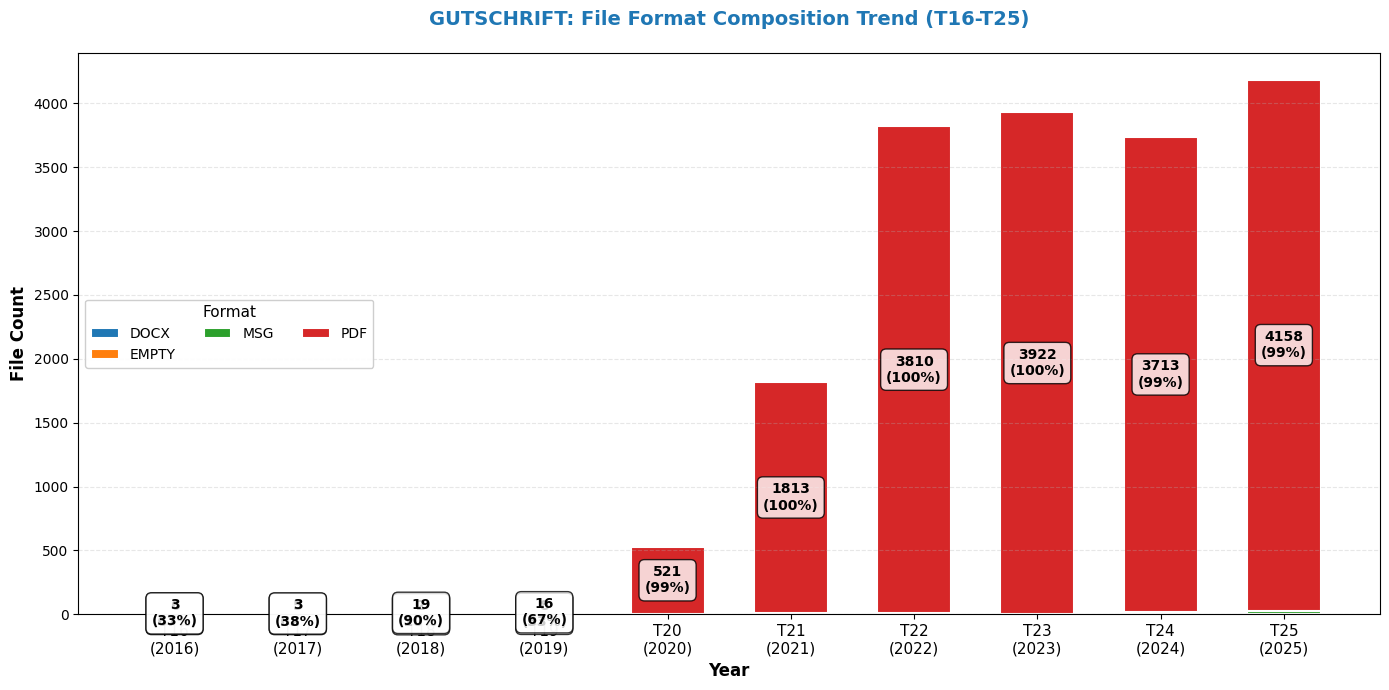
\includegraphics[width=\textwidth]{figures/gutschrift_file_format_trend.png}
    \caption[Gutschrift: file format composition trend]{Gutschrift: file format composition trend (2016 to 2025).}
    \label{fig:gs-trend}
\end{figure}

\begin{figure}[H]
    \centering
    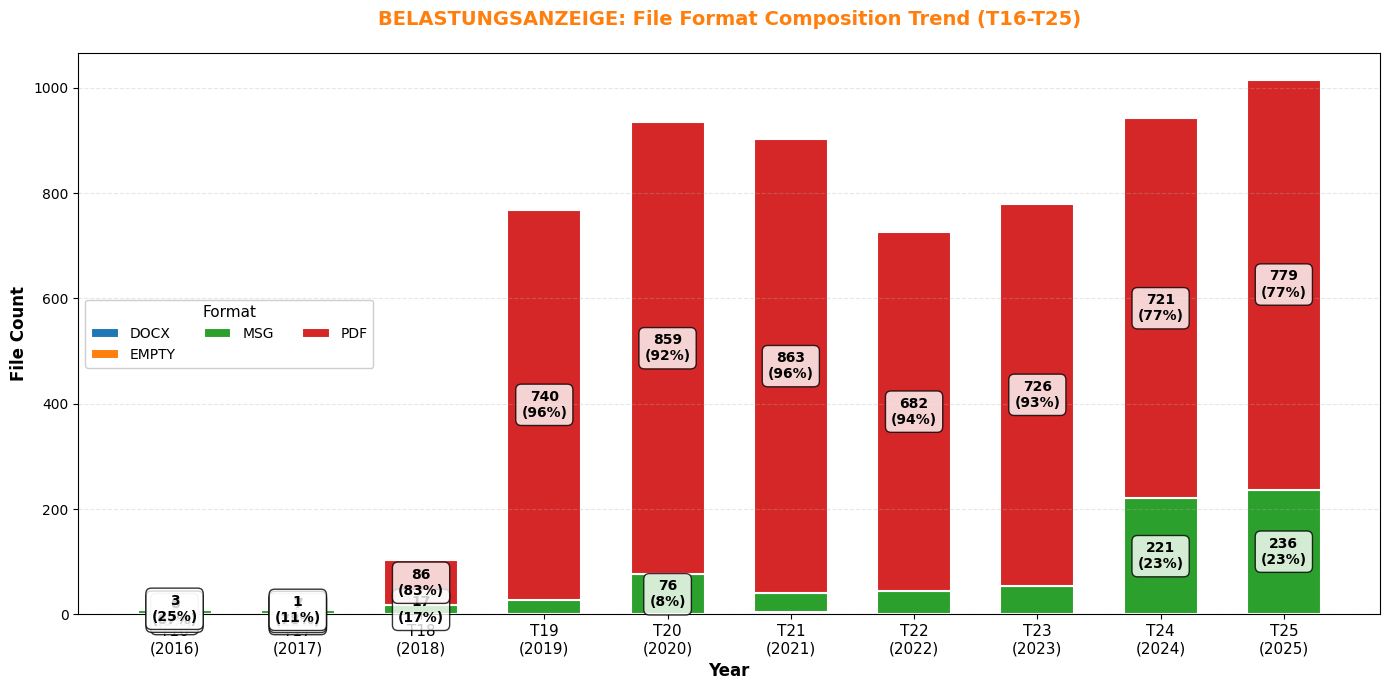
\includegraphics[width=\textwidth]{figures/belastungsanzeige_file_format_trend.png}
    \caption[Belastungsanzeige: file format composition trend]{Belastungsanzeige: file format composition trend (2016 to 2025).}
    \label{fig:bl-trend}
\end{figure}

\begin{figure}[H]
    \centering
    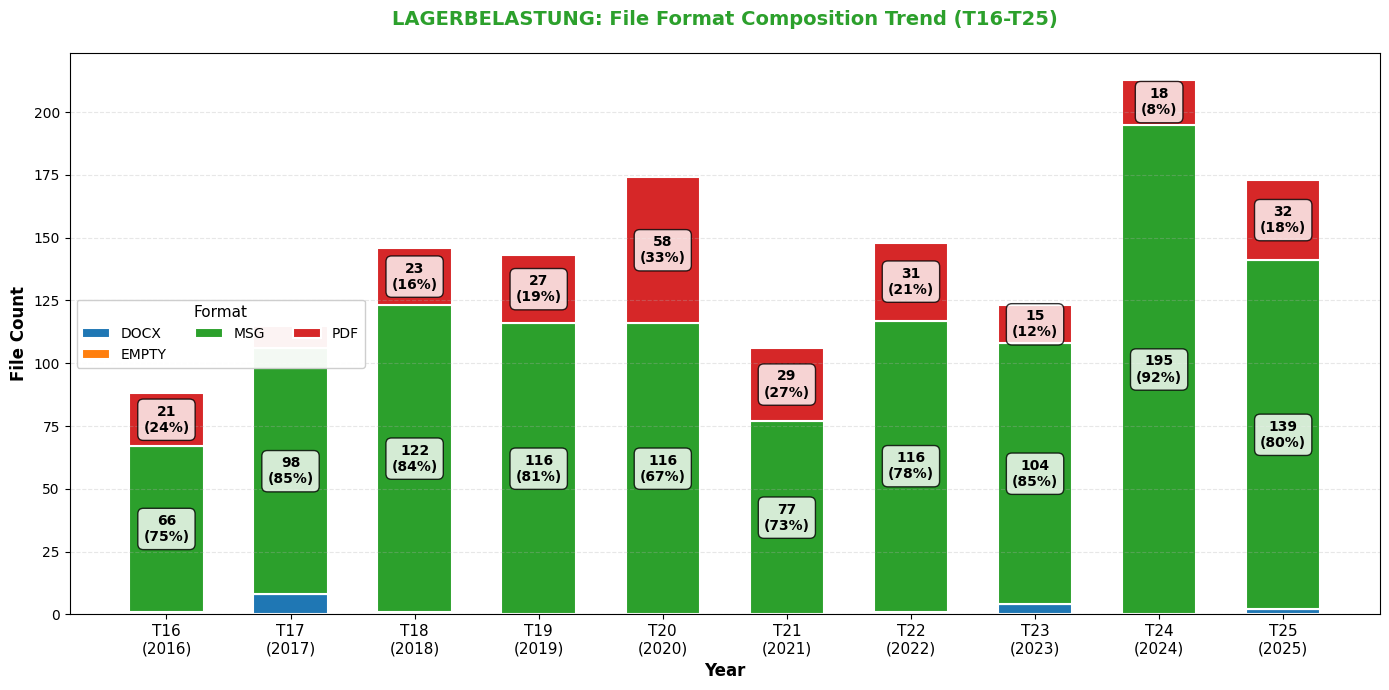
\includegraphics[width=\textwidth]{figures/lagerbelastung_file_format_trend.png}
    \caption[Lagerbelastung: file format composition trend]{Lagerbelastung: file format composition trend (2016 to 2025).}
    \label{fig:lb-trend}
\end{figure}

Figures~\ref{fig:gs-records}--\ref{fig:lb-records} show the number of
records per year for each category.  An important caveat applies to all of
these year-by-year figures: the data only becomes reliable from~2022 onwards.
Before that year, the company used a different process for recording and
archiving service tickets, so the lower record counts in the earlier years
reflect incomplete digital capture rather than a genuine absence of service
activity.  The sharp increase visible around 2021 and 2022 is therefore largely
an artefact of this process change, and any trend analysis should focus on the
period from 2022 onwards.

\begin{figure}[H]
    \centering
    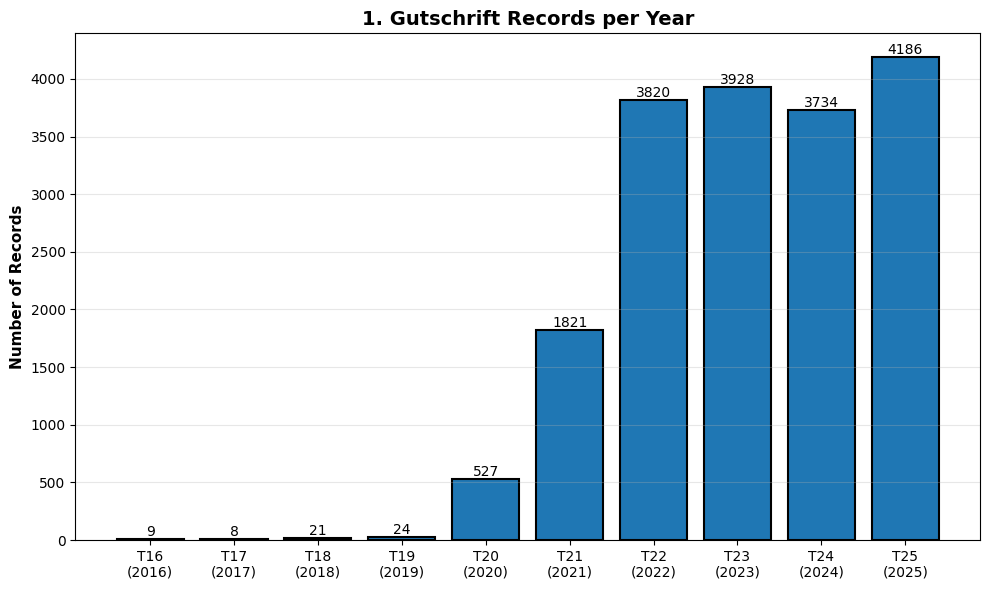
\includegraphics[width=\textwidth]{figures/gutschrift_records_per_year.png}
    \caption[Gutschrift records per year]{Gutschrift records per year (2016 to 2025). Data from 2022 onwards
             is reliable; earlier years are affected by a change in the
             company's recording process.}
    \label{fig:gs-records}
\end{figure}

\begin{figure}[H]
    \centering
    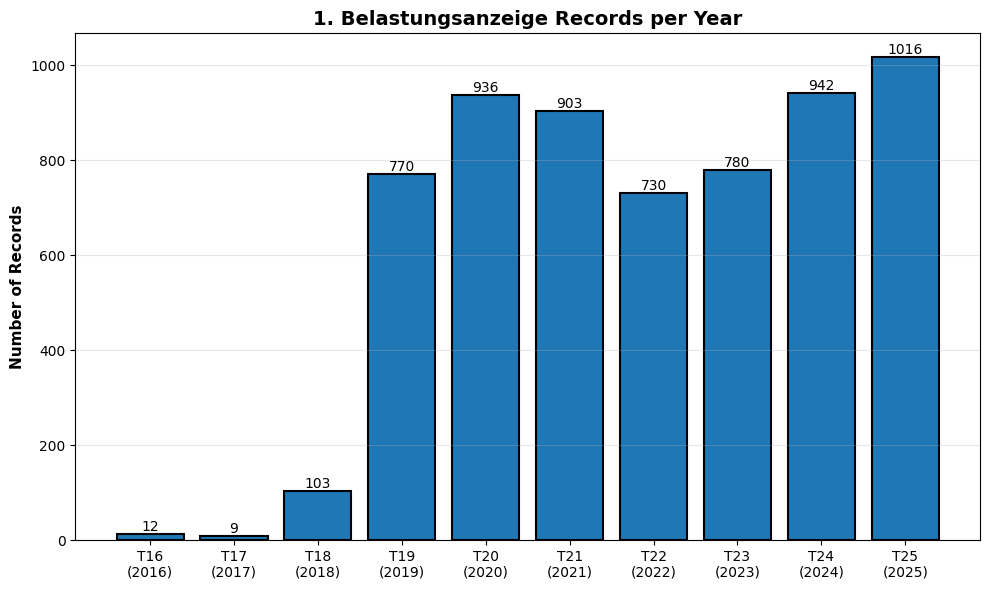
\includegraphics[width=\textwidth]{figures/belastungsanzeige_records_per_year.png}
    \caption[Belastungsanzeige records per year]{Belastungsanzeige records per year (2016 to 2025). Data from 2022
             onwards is reliable; earlier years are affected by a change in the
             company's recording process.}
    \label{fig:bl-records}
\end{figure}

\begin{figure}[H]
    \centering
    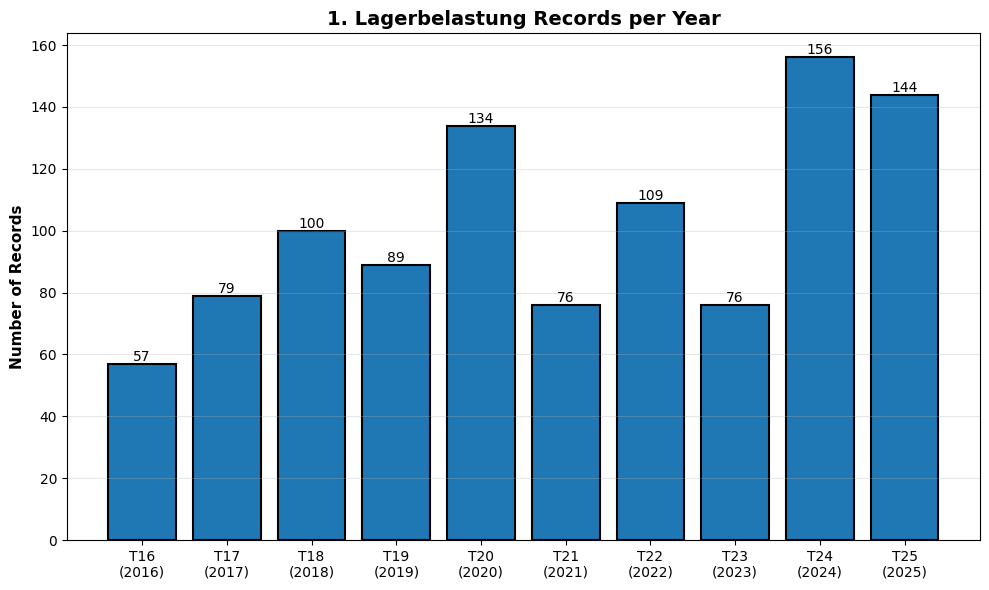
\includegraphics[width=\textwidth]{figures/lagerbelastung_records_per_year.png}
    \caption[Lagerbelastung records per year]{Lagerbelastung records per year (2016 to 2025). Data from 2022
             onwards is reliable; earlier years are affected by a change in the
             company's recording process.}
    \label{fig:lb-records}
\end{figure}

Figure~\ref{fig:gs-money} shows the total monetary value of Gutschrift
credit notes per year, peaking at over 9.1~million~EUR in 2023.
Figure~\ref{fig:bl-cost} shows the total cost per year for Belastungsanzeige
charge notifications.  The same reliability caveat applies: only the values
from~2022 onwards should be treated as representative.

\begin{figure}[H]
    \centering
    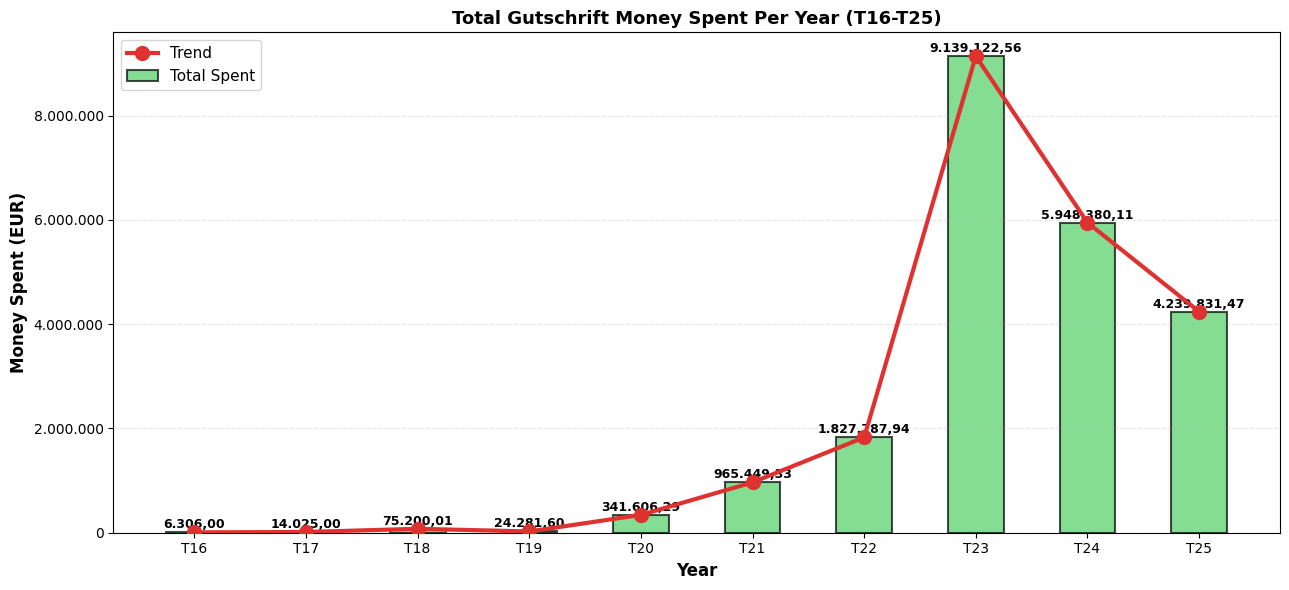
\includegraphics[width=\textwidth]{figures/gutschrift_money_spent.png}
    \caption[Total Gutschrift credit note value per year]{Total Gutschrift credit note value per year in EUR (2016 to 2025). The monetary values shown were extracted automatically with regular expressions and have not been independently verified.}
    \label{fig:gs-money}
\end{figure}

\begin{figure}[H]
    \centering
    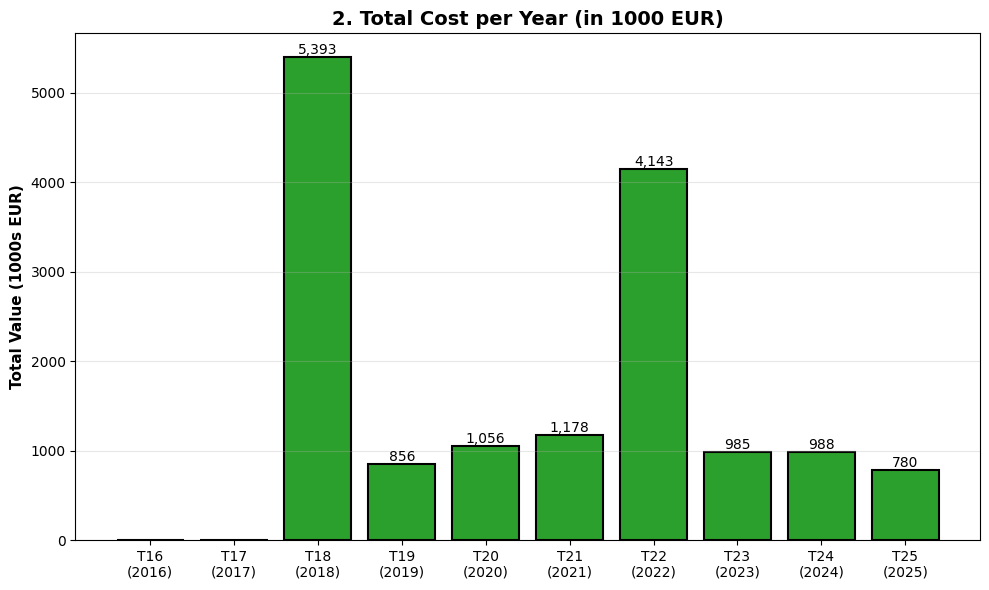
\includegraphics[width=\textwidth]{figures/belastungsanzeige_cost_per_year.png}
    \caption[Total Belastungsanzeige cost per year]{Total Belastungsanzeige cost per year in 1000~EUR (2016 to 2025). The monetary values shown were extracted automatically with regular expressions and have not been independently verified.}
    \label{fig:bl-cost}
\end{figure}

\subsection{File Conversion to Markdown}
%
All attachment types are converted to plain Markdown to create a uniform
input format for the LLM.  The conversion is performed by a custom pipeline
built for this thesis, which calls a dedicated library for each file type and
then post-processes the result.  The conversion strategy is:

\begin{itemize}
    \item MSG~(email) files: headers~(From, To, Subject, Date)
          are extracted and appended as a structured preamble, and the email body
          is normalised to plain text.  Nested reply chains are concatenated
          in chronological order (oldest first).  A custom filter in the
          pipeline removes quoted text in deep threads to reduce token
          redundancy; this filtering is part of the pipeline and is not done by
          any external conversion tool.

    \item PDF files: text is extracted using PyMuPDF4LLM, which
          preserves table structure and avoids common layout artefacts.
          Pages are separated by horizontal rules.  For scanned documents that
          contain no machine-readable text, the pipeline falls back to optical
          character recognition with Tesseract; this fallback is invoked by the
          pipeline itself, not by PyMuPDF4LLM.
\end{itemize}

\subsubsection{PDF Extraction Tool Selection}
%
The initial extraction attempts used MarkItDown~\cite{markitdown2024},
a general-purpose file-to-Markdown converter.  However, MarkItDown failed to
extract the ticket content in a correctly structured manner.  As shown in
Figure~\ref{fig:markitdown-drawback}, the converter linearises the document
into a flat sequence of fragments: column headers~(\texttt{POS},
\texttt{NO.\,D'ARTICLE}, \texttt{QUANT.}) are separated from their
corresponding values, and the tabular relationship between an article number,
its description, and its price is lost entirely.  Compared to the original PDF
layout, the extracted text is no longer
machine-interpretable as a structured invoice, which makes downstream entity
extraction unreliable.

\begin{figure}[H]
    \centering
    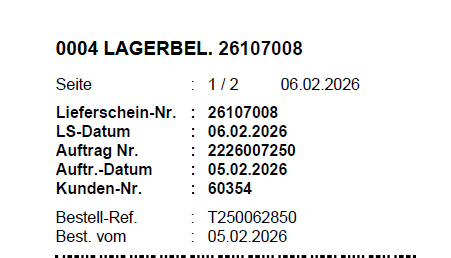
\includegraphics[width=0.82\textwidth]{figures/markitdown_drawback_output.png}\\[1ex]
    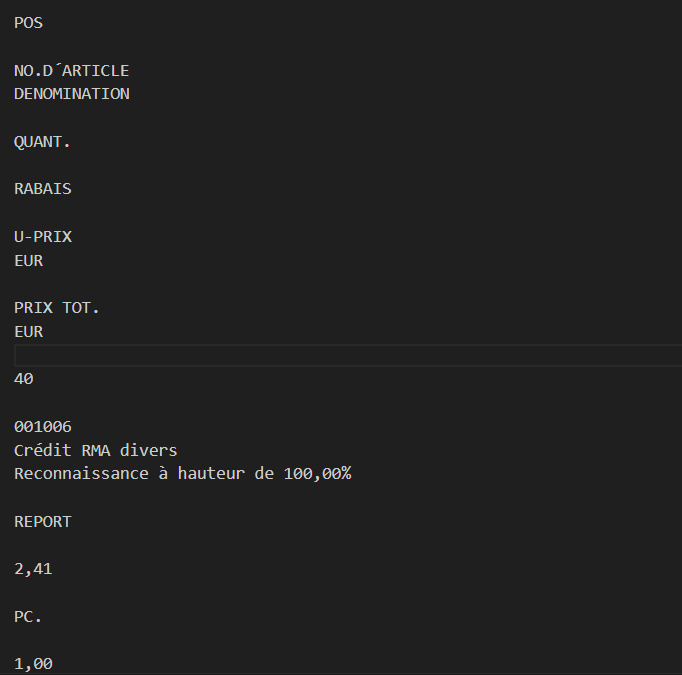
\includegraphics[width=0.82\textwidth]{figures/markitdown_drawback_original.png}
    \caption{Drawback of MarkItDown (example).  Top: the unstructured, linearised
             output, where table columns are detached from their values.
             Bottom: the original PDF layout that should have been preserved.
             These images are illustrative examples taken from one sample
             document.}
    \label{fig:markitdown-drawback}
\end{figure}

Motivated by this failure, four alternative libraries were evaluated on a test
set of 15~PDFs (5~Gutschrift, 5~Lagerbelastung, 5~Belastungsanzeige).  Before
presenting the comparison, it is worth briefly introducing these tools.  Tabula
is an open-source library specialised in detecting and extracting tables from
PDF documents.  Docling is an open-source document-conversion toolkit from IBM
that parses a PDF into a structured representation and exports it to Markdown or
JSON.  Spire.PDF is a commercial library for reading and manipulating PDF files,
including text and table extraction.  PyMuPDF4LLM is a wrapper around the PyMuPDF
engine that converts PDF pages to Markdown in a form intended for large language
model input.  A tool scores one point per PDF where \emph{all} expected fields
are correctly extracted.  Table~\ref{tab:tool-comparison} summarises the results.

\begin{table}[H]
    \centering
    \caption[PDF extraction tool comparison]{PDF extraction tool comparison (score: number of PDFs out of~15
             from which all expected fields were correctly extracted).}
    \label{tab:tool-comparison}
    \begin{tabular}{llcl}
        \hline
        \textbf{Library} & \textbf{License} & \textbf{Score} & \textbf{Cost} \\
        \hline
        PyMuPDF4LLM & AGPL       & \textbf{15/15} & Free (if not hosted) \\
        Docling      & MIT        & 11/15          & Free \\
        Spire        & Commercial & 11/15          & Paid \\
        Tabula-py    & MIT        & 6/15           & Free \\
        \hline
    \end{tabular}
\end{table}

Each tool exhibited a characteristic failure mode:

\begin{itemize}
    \item Tabula (6/15).  Tabula is specialised for table extraction
          and performed well \emph{only} on the tabular regions of a document.
          As shown in Figure~\ref{fig:tool-tabula}, it correctly reconstructs
          the key-value table~(Lieferschein-Nr., LS-Datum, Auftrag~Nr.) but
          populates many cells with \texttt{nan} and ignores all
          non-tabular text, so most documents were only partially captured.

    \item Docling (11/15).  Docling produced output that was often
          similar to the unstructured MarkItDown result.  As shown in
          Figure~\ref{fig:tool-docling}, when configured for table extraction
          it linearised the fields into separate lines and, on the 5~test PDFs
          checked specifically for table fidelity, it missed the tables in CSV
          form.

    \item Spire (11/15).  Spire matched Docling's score but, like
          MarkItDown, frequently returned a flat, unstructured stream of
          values~(Figure~\ref{fig:tool-spire}).  It is also a commercial,
          paid library.

    \item PyMuPDF4LLM (15/15).  PyMuPDF4LLM~\cite{pymupdf4llm} was the
          only tool to achieve a perfect score across all three document
          categories.  As shown in Figure~\ref{fig:tool-pymupdf4llm}, it
          preserves both the header block and the tabular structure as proper
          Markdown tables, keeping article numbers, descriptions, and prices in
          their correct relationship.
\end{itemize}

\begin{figure}[H]
    \centering
    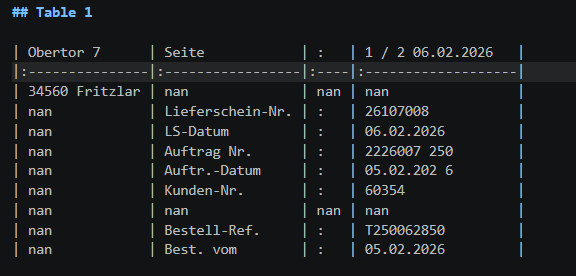
\includegraphics[width=0.92\textwidth]{figures/tool_tabula.png}
    \caption{Tabula output. Tables are reconstructed but many cells are
             \texttt{nan} and non-tabular text is dropped.}
    \label{fig:tool-tabula}
\end{figure}

\begin{figure}[H]
    \centering
    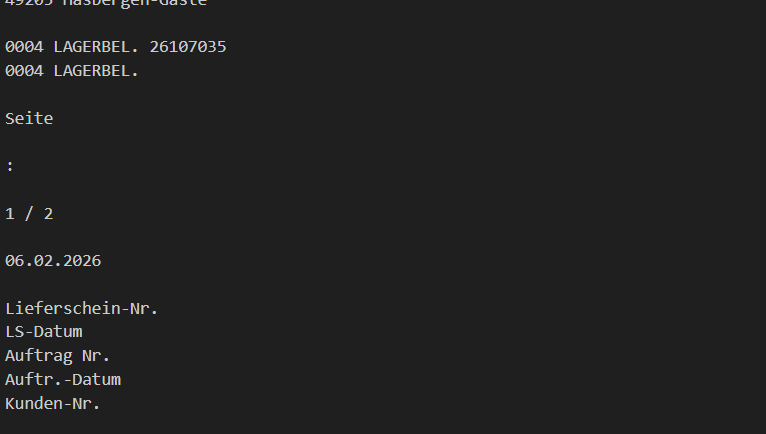
\includegraphics[width=0.92\textwidth]{figures/tool_docling.png}
    \caption{Docling output. Fields are linearised and table structure
             is lost when exporting to CSV.}
    \label{fig:tool-docling}
\end{figure}

\begin{figure}[H]
    \centering
    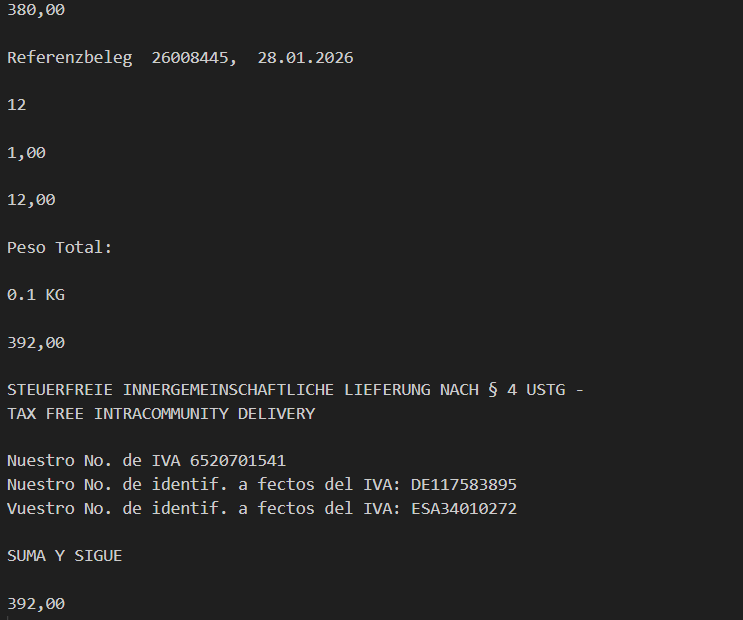
\includegraphics[width=0.85\textwidth]{figures/tool_spire.png}
    \caption{Spire output. A flat, unstructured stream of values
             similar to MarkItDown.}
    \label{fig:tool-spire}
\end{figure}

\begin{figure}[H]
    \centering
    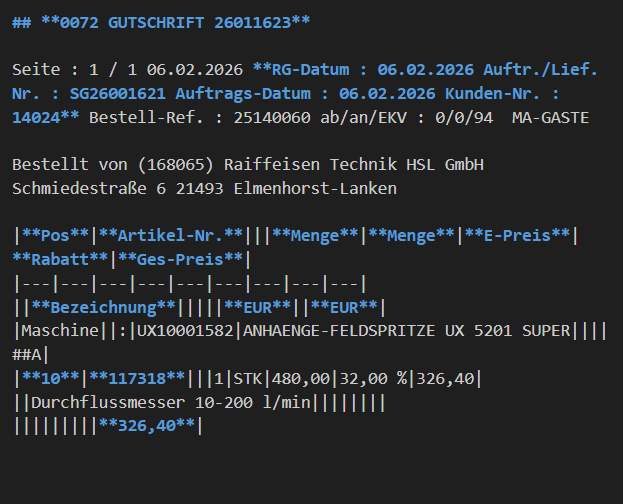
\includegraphics[width=0.92\textwidth]{figures/tool_pymupdf4llm.png}
    \caption{PyMuPDF4LLM output. Header block and tabular structure are
             preserved as proper Markdown tables.}
    \label{fig:tool-pymupdf4llm}
\end{figure}

Based on this comparison, PyMuPDF4LLM was selected as the PDF extraction tool
for the entire pipeline.  Files that cannot be converted~(corrupted,
password-protected, image-only PDFs) are skipped and logged; the remaining text
files are combined into a single \texttt{.msg.md} file per ticket.

\subsection{Token Budget Management and Cleaning}
\label{subsec:cleaning}
%
Given the 128k context window of the target models, most email threads fit
entirely.  However, to improve reasoning performance and reduce noise, a
cleaning pass is applied.  The following boilerplate patterns were identified
and removed automatically:

\begin{table}[H]
    \centering
    \caption{Most frequent boilerplate patterns removed during preprocessing.}
    \label{tab:boilerplate}
    \begin{tabular}{lr}
        \hline
        \textbf{Pattern} & \textbf{Files affected} \\
        \hline
        KG Legal Footer             & 86,408 \\
        Bank Details Block          & 84,108 \\
        AMAZONE Postal Header       & 78,073 \\
        Manufacturer Header         & 69,074 \\
        OS Trademark Notice         & 17,516 \\
        AMAZONE Standalone Address  & 13,304 \\
        urldefense URL              & 12,099 \\
        SafeLinks URL               &  8,323 \\
        IBAN Lines                  &  5,144 \\
        AMAZONE GDPR Notice DE      &  2,860 \\
        \hline
    \end{tabular}
\end{table}

\noindent
The pattern names in Table~\ref{tab:boilerplate} refer to recurring blocks of
text that were observed repeatedly across the corpus and carry no
ticket-specific information.  For example, the \emph{KG Legal Footer} is the
standard company legal footer (the firm's full legal name and registration
details) that appears at the bottom of almost every document, the \emph{Bank
Details Block} is the recurring bank-account section, and the \emph{AMAZONE
Postal Header} is the fixed sender address line.  These blocks were identified
by inspecting the most frequent repeated text segments in the benchmark data and
were removed automatically so that they do not consume context or add noise.

The combined preprocessing results are:

\begin{table}[H]
    \centering
    \caption{Preprocessing compression results.}
    \label{tab:compression}
    \begin{tabular}{lr}
        \hline
        \textbf{Metric} & \textbf{Value} \\
        \hline
        Files scanned        & 242,499 \\
        Image-only deleted   & 11,917 \\
        Files compressed     & 216,246 \\
        Files unchanged      & 14,336 \\
        Errors               & 0 \\
        \hline
        Original size        & 949.9\,MB \\
        Space saved          & 219.5\,MB \\
        Reduction            & 23.1\% \\
        \hline
    \end{tabular}
\end{table}

\subsection{Rule-based Pattern Extraction}
\label{subsec:regex}
%
An analysis of the documents revealed three recurring structured document
categories that can be identified reliably with regular expressions.  Because
the corpus is multilingual, the classifier does not rely on a single German
keyword but on a list of category keywords in several languages, combined with a
filename heuristic.  A document is assigned to a category if either its filename
matches a category-specific pattern or its first part matches a content pattern
built from the multilingual keyword list.

\begin{description}
    \item[Gutschrift~(Credit Note):] the filename pattern is
          \verb|gutschrift|credit.*note|, and the content pattern requires a
          four-digit number followed by a credit-note keyword such as
          \texttt{GUTSCHRIFT}, \texttt{CREDIT NOTE}, \texttt{NOTE DE
          CR\'EDIT}, \texttt{NOTA DI CREDITO}, or their equivalents in the
          other corpus languages.

    \item[Belastungsanzeige~(Charge Notification):] the filename pattern is
          \verb|belastung|debit.*note|, and the content pattern matches a
          debit-note keyword such as \texttt{BELASTUNGSANZEIGE}, \texttt{DEBIT
          NOTE}, \texttt{NOTE DE D\'EBIT}, or \texttt{NOTA DI ADDEBITO}.

    \item[Lagerbelastung~(Warehouse Charge):] the filename pattern is
          \verb|lagerbelastung|lager|warehouse.*debit|stock.*debit|, and the
          content pattern matches a stock-charge keyword such as
          \texttt{LAGERBELASTUNG}, \texttt{STOCK DEBIT}, or \texttt{WAREHOUSE
          DEBIT}.
\end{description}

The monetary total of a document is captured with a dedicated pattern that
looks for a total-value label such as \texttt{Gesamtwert}, \texttt{Total},
\texttt{Montant total}, or \texttt{Valor total}, followed within a short window
by a currency amount.  The amount is then parsed from the European number
format~(for example \texttt{1.234,56}) into a numeric value.

Beyond document-category detection and totals, the pipeline extracts the
identifiers that follow predictable patterns:

\begin{itemize}
    \item Machine serial numbers, matched by prefixed digit patterns such as
          \verb|UX\d{7,}| and \verb|CYA\d{7,}|.
    \item Article numbers, matched as digit sequences appearing in a part-list
          context.
    \item Change numbers~(Anderungsnummer), matched by \verb|CN[A-Z]?\d{4,}|,
          which also captures variants such as \texttt{CNY0001440}.
\end{itemize}

This rule-based layer addresses RQ\,1.1 directly: structured, pattern-conformant
information is captured without an LLM.  The LLM is reserved for extracting
the semantic tags from the narrative text.

\subsection{Item Extraction}
\label{subsec:item-extraction}
%
Applying the rule-based layer to the full corpus produces a structured record of
the items mentioned in each document.  Three kinds of identifier are of
particular interest: the article numbers (Artikel-Nr.), the customer's own part
number (Ihre Teilenummer), and the change numbers (Anderungsnummer, prefixed
with \texttt{CN}).  Because the three document categories follow different
layouts, these identifiers are stored in slightly different fields per category:
the Gutschrift and Lagerbelastung documents expose a single list of article
numbers, whereas the Belastungsanzeige documents separate the internal part
number from the customer's own part number.

Table~\ref{tab:item-extraction} summarises the volume of extracted identifiers.
The Gutschrift category dominates the article counts, with a single article
number (\texttt{0520700}) appearing more than 88{,}000 times, which reflects a
small number of very high-volume spare parts.  The change numbers are far less
frequent but are operationally important, since they link a ticket to a specific
engineering change.

\begin{table}[H]
    \centering
    \caption[Volume of extracted items per category]{Volume of extracted items per category. Article numbers, customer part numbers, and change numbers (CN) after applying the length and pattern filters.}
    \label{tab:item-extraction}
    \begin{tabular}{lrrrr}
        \hline
        \textbf{Category} & \textbf{Articles} & \textbf{Unique articles} & \textbf{CN total} & \textbf{CN unique} \\
        \hline
        Gutschrift        & 327{,}763 & 18{,}101 & 1{,}775 & 623 \\
        Belastungsanzeige &   4{,}868 &  1{,}537 & 3{,}288 & 934 \\
        Lagerbelastung    &   1{,}960 &  1{,}417 &       0 &   0 \\
        \hline
    \end{tabular}
\end{table}

Figure~\ref{fig:item-articles} shows the twenty most frequent article numbers in
each category.  The distribution is highly skewed for Gutschrift, where a few
standard parts account for the bulk of all occurrences, and much flatter for
Lagerbelastung, where no single part dominates.

\begin{figure}[H]
    \centering
    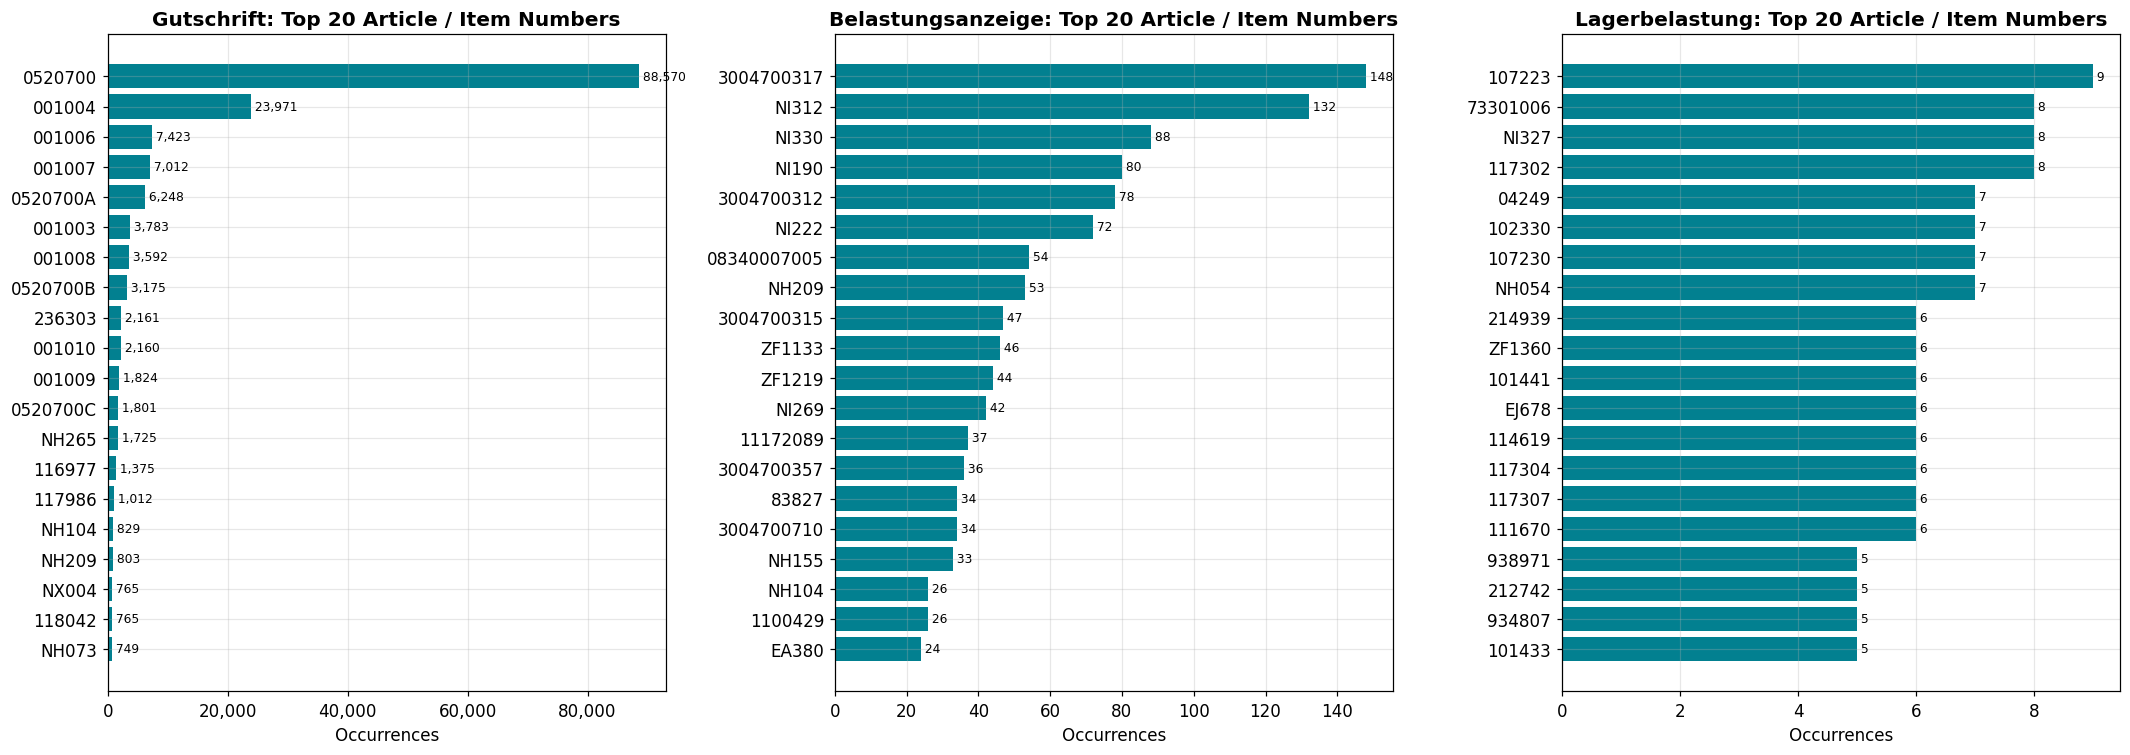
\includegraphics[width=\textwidth]{figures/fig_top_article_numbers.png}
    \caption[Top article numbers per category]{Top twenty article and item numbers per category, after filtering out change numbers and short tokens.}
    \label{fig:item-articles}
\end{figure}

For the Belastungsanzeige category, the customer's own part number is recorded in
a dedicated field.  Figure~\ref{fig:item-ihre} shows the most frequent values,
which are useful for tracing recurring customer-side components.

\begin{figure}[H]
    \centering
    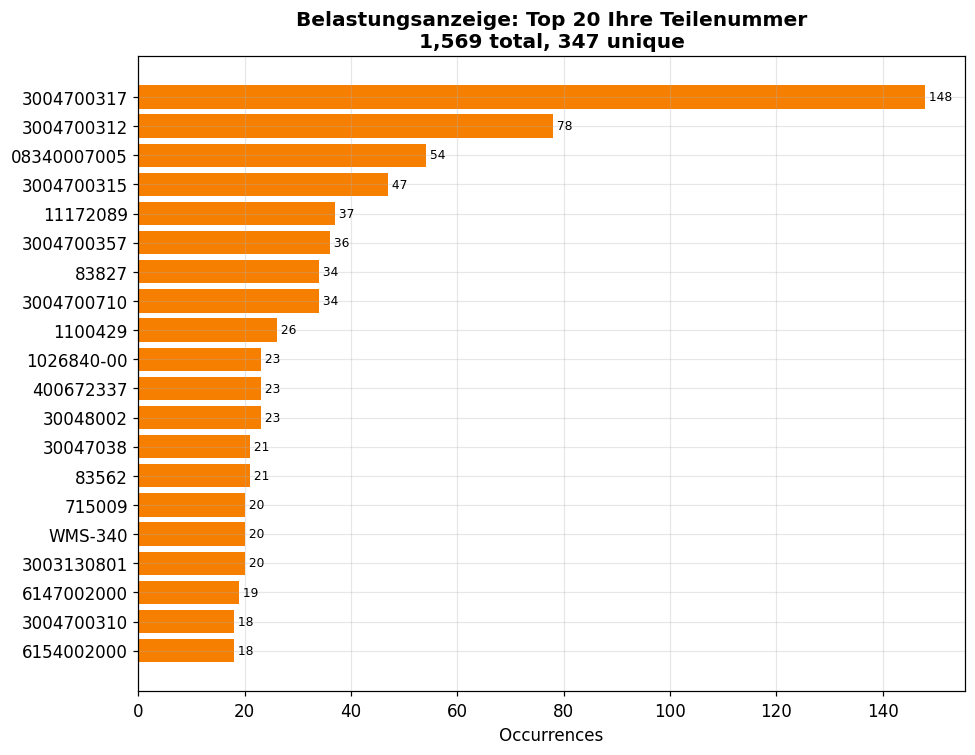
\includegraphics[width=0.78\textwidth]{figures/fig_ihre_teilenummer.png}
    \caption[Top customer part numbers]{Top twenty customer part numbers (Ihre Teilenummer) in the Belastungsanzeige category.}
    \label{fig:item-ihre}
\end{figure}

The change numbers are extracted separately and, as
Figure~\ref{fig:item-cn} shows, the sets found in the Gutschrift and
Belastungsanzeige categories are almost entirely disjoint: of the several
hundred unique change numbers in each category, only a single number appears in
both.  They are therefore presented as two separate distributions rather than a
combined one.  It is worth noting that in the Gutschrift documents the change
numbers were not isolated in a dedicated field but had to be recovered from the
surrounding text, which is a limitation of the original extraction and a
candidate for future refinement.

\begin{figure}[H]
    \centering
    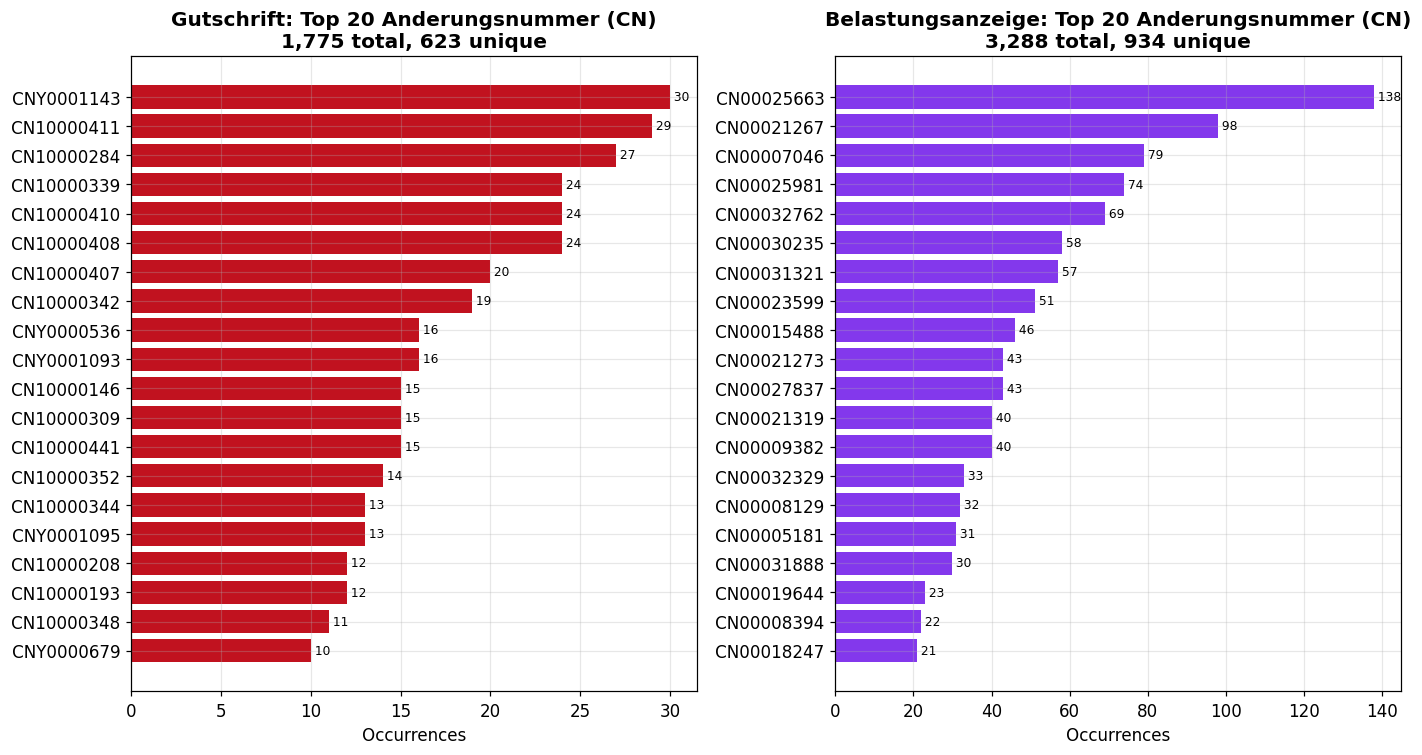
\includegraphics[width=\textwidth]{figures/fig_anderungsnummer.png}
    \caption[Change number occurrences per category]{Top twenty change numbers (Anderungsnummer, CN) for the Gutschrift and Belastungsanzeige categories, shown separately because the two sets are disjoint.}
    \label{fig:item-cn}
\end{figure}

%----------------------------------------------------------------------
\section{Benchmark Dataset and Validation}
\label{sec:benchmark}
%
\subsection{Ticket Selection}
%
A stratified sample of 250~tickets was drawn from the full corpus to represent
three distinct ticket categories:

\begin{itemize}
    \item \textbf{GS~(Gutschrift/Credit-note tickets):} Billing corrections,
          credit requests, invoice disputes.
    \item \textbf{BL~(Belastungsanzeige tickets):} Charge notifications,
          commission corrections, return-goods authorisations.
    \item \textbf{LB~(Lagerbelastung tickets):} Warehouse charges,
          stock adjustments, logistics issues.
\end{itemize}

Tickets were selected to ensure coverage of different years~(2016 to 2025),
a variety of email-thread lengths~(1 to 20+ messages), and both resolved and
unresolved cases.  The benchmark composition is 50~Gutschrift,
100~Belastungsanzeige, and 100~Lagerbelastung tickets, chosen to balance
category representation with the relative complexity of each type.

\subsubsection{Benchmark Data Characteristics}
%
The language distribution of the benchmark tickets is dominated by German
(Table~\ref{tab:language-dist}), reflecting the typical communication
patterns between Amazone's German headquarters and its international
dealer network.

\begin{table}[H]
    \centering
    \caption{Language distribution across the source files in the 250-ticket benchmark.}
    \label{tab:language-dist}
    \begin{tabular}{lrr}
        \hline
        \textbf{Language} & \textbf{Percent} & \textbf{Files} \\
        \hline
        German   & 82.8\% & 538 \\
        English  & 15.7\% & 102 \\
        Russian  &  1.1\% &   7 \\
        Spanish  &  0.3\% &   2 \\
        Estonian &  0.2\% &   1 \\
        \hline
    \end{tabular}
\end{table}

\noindent
The counts in Table~\ref{tab:language-dist} refer to individual source files,
not tickets: a single ticket bundles several files, so the file counts exceed
the 250 tickets.  German and English together account for the overwhelming
majority, with a small remainder in Russian, Spanish, and Estonian.

Figure~\ref{fig:benchmark-filetypes} shows the distribution of source file
types in the benchmark.  MSG email files dominate overwhelmingly (622~out of
650~files, 95.7\%), confirming that the primary communication channel is
email.

\begin{figure}[H]
    \centering
    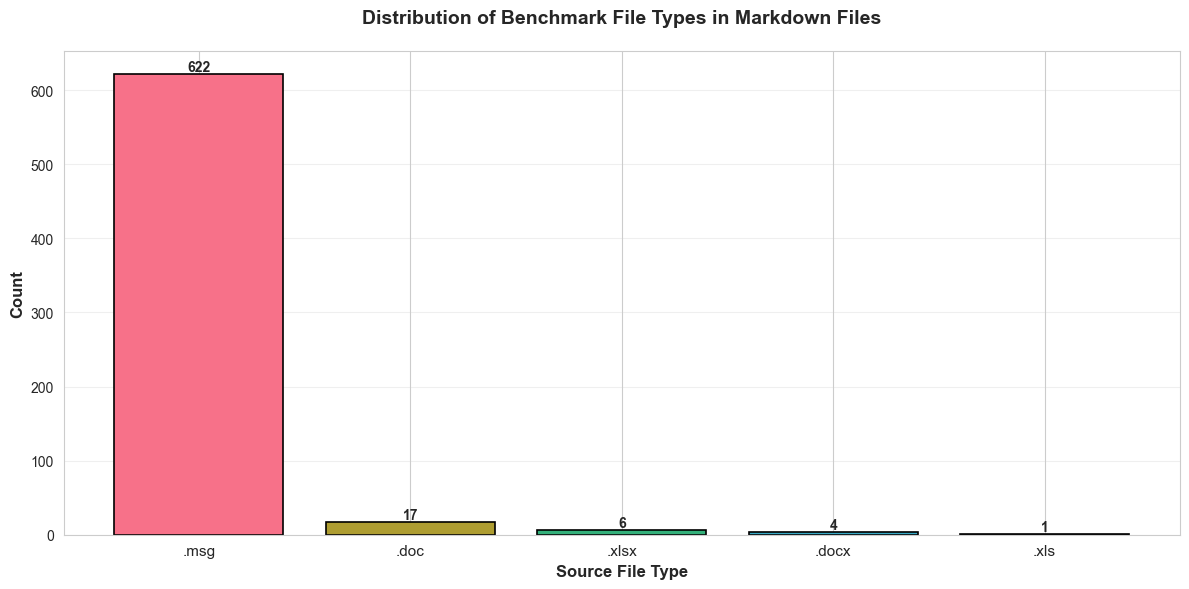
\includegraphics[width=\textwidth]{figures/benchmark_file_type_distribution.png}
    \caption{Distribution of source file types in the benchmark Markdown files.}
    \label{fig:benchmark-filetypes}
\end{figure}

Figure~\ref{fig:ticket-classification} shows that 237~tickets~(97.1\%)
contain at least one \texttt{.msg.md} file, while only 7~tickets~(2.9\%)
consist entirely of non-email files.

\begin{figure}[H]
    \centering
    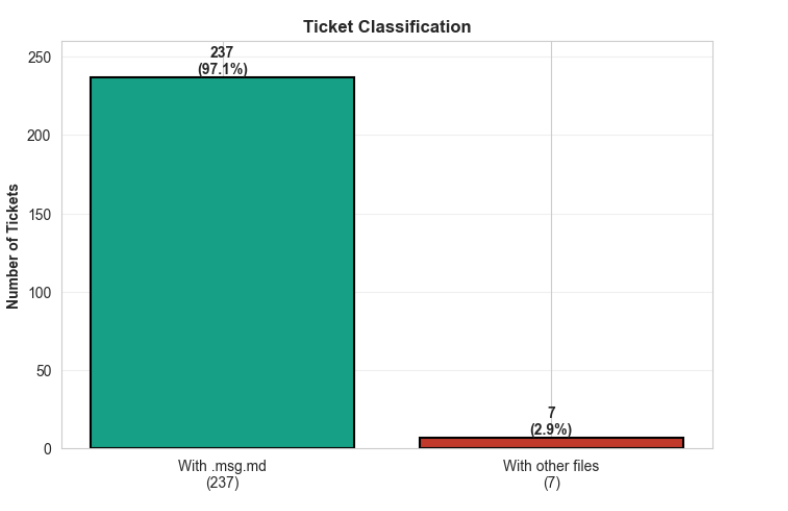
\includegraphics[width=0.95\textwidth]{figures/ticket_classification.png}
    \caption{Ticket classification: tickets with .msg.md files vs other files only.}
    \label{fig:ticket-classification}
\end{figure}

Figure~\ref{fig:files-per-ticket} shows the distribution of files per
ticket.  The majority of tickets (60.7\%) contain only a single file, while
4.9\% contain eleven or more files, representing complex multi-message
threads with attachments.

\begin{figure}[H]
    \centering
    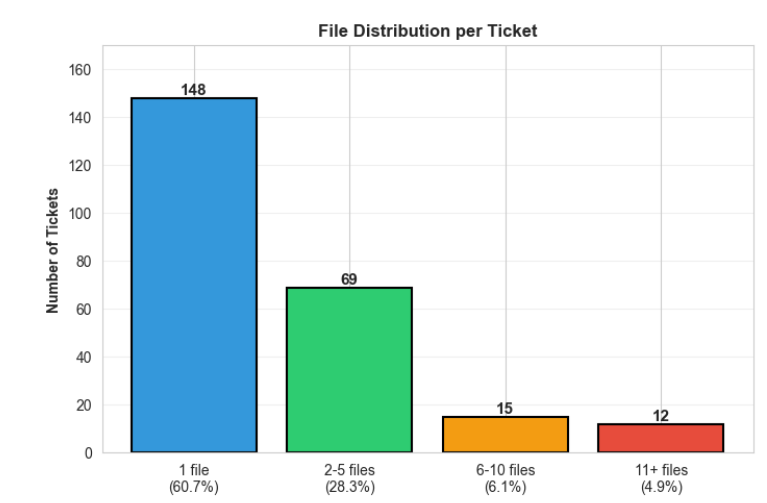
\includegraphics[width=\textwidth]{figures/file_distribution_per_ticket.png}
    \caption{Distribution of files per ticket in the benchmark dataset.}
    \label{fig:files-per-ticket}
\end{figure}

\subsection{Human Annotation}
%
Each ticket was annotated by a single domain expert with knowledge of
Amazone's service operations.  The annotation task consisted of assigning
1 to 4 tags to each ticket from a curated set of 28 human-defined tags, for
example \texttt{kulanz}, \texttt{wrong\_booking}, and \texttt{discussion}.

These 28~tags form the human-annotated ground truth used in the F1 evaluation.
They were developed manually by working through the benchmark tickets and
grouping the most common and clearly recurring service themes into reusable
labels.  The tags are intentionally coarse-grained and service-action-oriented
to maximise reusability across similar tickets.

This human-defined set was later extended into a larger taxonomy of
126~tags for the blind tag evaluation.  The extension was driven by the
language models themselves: prompting the models to generate tags freely across
the corpus produced a pool of roughly 1{,}789~candidate tags, which was then
reduced to 126~clear, non-overlapping labels through a dedicated
quality-control pass.  The full development process is described in
Section~\ref{sec:disc-tags}, and the complete 126-tag list is provided in
Appendix~\ref{chap:TagTaxonomy}.

\subsection{Annotation Quality}
%
Inter-annotator agreement was not formally measured for the full benchmark
because only one annotator was available.  However, a reliability check was
performed on 25~tickets~(10\,\% of the benchmark), where the annotator
re-labelled the same tickets two weeks after the initial annotation.
The self-agreement F1 was \(0.88\), indicating good consistency.

%----------------------------------------------------------------------
\section{LLM Setup and Prompt Design}
\label{sec:llm-setup}
%
\subsection{Model Serving Infrastructure}
%
All open-source models are served via \textbf{Ollama}~(v0.3), a lightweight
local inference server, on a dedicated GPU server~(\texttt{ve-ds-nns-01}).
The server is equipped with sufficient VRAM to run 8B to 20B parameter models
at 4-bit quantisation.  The OpenWebUI front-end is used for interactive
testing and context-window verification.

The proprietary models~(GPT-4o, GPT-3.5-Turbo, GPT-4o-mini) are accessed via
the OpenAI API.

\subsection{Models Evaluated}
%
Table~\ref{tab:models} lists all fifteen model configurations evaluated in
this thesis, spanning both open-source models served via Ollama and
proprietary models accessed via the OpenAI API.

\begin{table}[H]
    \centering
    \caption{Models evaluated in the benchmark study.}
    \label{tab:models}
    \begin{tabular}{llll}
        \hline
        \textbf{Short Name} & \textbf{Model} & \textbf{Source} & \textbf{Origin} \\
        \hline
        gptoss         & gpt-oss:20b          & Ollama  & OpenAI (USA) \\
        gemma4         & gemma4:7b             & Ollama  & Google (USA) \\
        gemma7b        & gemma:7b              & Ollama  & Google (USA) \\
        llama3.1       & llama3.1:8b           & Ollama  & Meta (USA) \\
        llama3.2       & llama3.2:latest       & Ollama  & Meta (USA) \\
        dolphin        & dolphin-mixtral       & Ollama  & Mistral AI (France) \\
        qwen3\_14b     & qwen3:14b             & Ollama  & Alibaba (China) \\
        qwen2.5        & qwen2.5:7b            & Ollama  & Alibaba (China) \\
        deepseek7b     & deepseek-r1:7b        & Ollama  & DeepSeek (China) \\
        deepseek14     & deepseek-r1:14b       & Ollama  & DeepSeek (China) \\
        gpt-5.5        & gpt-5.5               & API     & OpenAI (USA) \\
        gpt-5\_4-mini  & gpt-5.4-mini          & API     & OpenAI (USA) \\
        gpt-4o         & gpt-4o                & API     & OpenAI (USA) \\
        gpt-4o-mini    & gpt-4o-mini           & API     & OpenAI (USA) \\
        gpt-3.5-turbo  & gpt-3.5-turbo         & API     & OpenAI (USA) \\
        \hline
    \end{tabular}
\end{table}

Throughout this thesis, models are referred to by their Ollama identifier in
typewriter font, which combines the model family, its version, and its
parameter size, for example \texttt{gemma4:7b} or \texttt{deepseek-r1:14b}.
Where the parameter size is given separately, it appears in parentheses, as in
\texttt{gemma3 (12b)}.  It is important to note that the family version and the
parameter size are independent: \texttt{gemma4} and \texttt{gemma3 (12b)} are
two distinct model releases, not the same model written two ways.  This naming
convention is used consistently so that every result can be traced back to the
exact model that produced it.

\subsection{Prompt Design}
\label{sec:prompt-design}
%
Each ticket is processed with \textbf{two sequential API calls}:

\begin{enumerate}
    \item \textbf{Extraction call.}  The model receives the full ticket text
          and is instructed to return a JSON object with three fields:
          \texttt{Problem}~(one to two sentences), \texttt{Solution}~(one to two sentences),
          and \texttt{items}~(a JSON array of typed entity references).
          The prompt embeds explicit reasoning steps~(identify the problem,
          search for a solution, extract entities) to guide chain-of-thought
          processing.

    \item \textbf{Tagging call.}  The model receives the same ticket text and
          is instructed to return a JSON object with a \texttt{tags} array
          and a \texttt{reasoning} dictionary.  Tags must be drawn exclusively
          from the approved tag list; the model is penalised in the evaluation
          for invented tags.
\end{enumerate}

All prompts are written in English regardless of the ticket language.  The
instruction to output in English is repeated explicitly to counteract
the tendency of some models to mirror the input language.

Inference parameters are fixed across all models: temperature~$= 0.7$,
\texttt{num\_ctx}~$= 131{,}072$~tokens~(128k), \texttt{num\_predict}~$= 4{,}096$
tokens.  These values ensure that even the longest email threads are fully
ingested, while the output budget is generous enough to accommodate detailed
reasoning without being wastefully large.

%----------------------------------------------------------------------
\section{Experimental Protocol}
\label{sec:experimental-protocol}
%
\subsection{Pipeline Implementation}
%
The core pipeline is implemented as a single Python~3 script~(\texttt{extraction.py}).
For each row in the 250-ticket benchmark CSV, the script:

\begin{enumerate}
    \item Locates the ticket folder by matching the \texttt{parent\_name} and
          \texttt{ticket\_number} columns to the folder hierarchy on disk.
    \item Concatenates all \texttt{.msg.md} files for that ticket into one
          context string, prefixing each file's content with a
          \verb|[FILE: <name>]| header to preserve authorship context.
    \item Sends the extraction call and then the tagging call to the Ollama
          API, parses both JSON responses, and writes the results back to the
          output CSV.
    \item Saves a checkpoint every~10~rows~(\texttt{SAVE\_EVERY~=~10}) to
          prevent data loss on interruption.
\end{enumerate}

A one-second sleep is inserted between rows to reduce load on the GPU
server~\texttt{ve-ds-nns-01:11434}.

\chapter{Results}
%
\label{chap:Results}
%
This chapter presents the quantitative and qualitative results of the two
evaluation protocols described in Chapter~\ref{chap:Methodology}.
Section~\ref{sec:res-f1} reports token-level F1 scores from the blind tag
evaluation.  Section~\ref{sec:res-judge} presents the LLM-as-judge ratings.
Section~\ref{sec:res-oss} compares the open-source models,
Section~\ref{sec:res-fullrun} discusses the full-corpus run with the
best-performing configuration, and Section~\ref{sec:observations} summarises
cross-cutting observations.

%----------------------------------------------------------------------
\section{Blind Tag Evaluation -- F1 Scores}
\label{sec:res-f1}
%
\subsection{Per-Category and Overall F1}
%
Table~\ref{tab:f1-results} summarises the token-level F1 scores for all ten
model configurations across the three ticket categories.  All scores shown
are macro-averaged over the 250~benchmark tickets.

\begin{table}[htbp]
    \centering
    \caption{Token-level F1 scores on the blind tag benchmark (macro-average).
             Best result in each column is \textbf{bold}.}
    \label{tab:f1-results}
    \begin{tabular}{lcccc}
        \hline
        \textbf{Model} & \textbf{GS} & \textbf{BL} & \textbf{LB} & \textbf{Overall} \\
        \hline
        gpt-oss:20b         & \textbf{0.412} & \textbf{0.384} & \textbf{0.342} & \textbf{0.393} \\
        deepseek-r1:14b     & 0.385          & 0.362          & 0.321          & 0.368 \\
        qwen3:14b           & 0.372          & 0.351          & 0.315          & 0.356 \\
        gemma4:26b          & 0.364          & 0.342          & 0.302          & 0.345 \\
        llama3.1:8b         & 0.351          & 0.328          & 0.284          & 0.331 \\
        gemma4:latest       & 0.342          & 0.315          & 0.276          & 0.322 \\
        gpt-4o              & 0.391          & 0.371          & 0.334          & 0.376 \\
        gpt-4o-mini         & 0.365          & 0.348          & 0.298          & 0.348 \\
        gpt-3.5-turbo       & 0.321          & 0.294          & 0.245          & 0.298 \\
        llama3.2:3b         & 0.284          & 0.251          & 0.212          & 0.259 \\
        \hline
    \end{tabular}
\end{table}

\subsection{Performance of Rule-based Extraction (RQ1)}
\label{subsec:regex-res}
%
Table~\ref{tab:regex-results} shows the performance of the regular expression
patterns described in Section~\ref{subsec:regex} for structured field
extraction.

\begin{table}[htbp]
    \centering
    \caption{Performance of regex patterns for structured extraction.}
    \label{tab:regex-results}
    \begin{tabular}{lccc}
        \hline
        \textbf{Field Type} & \textbf{Precision} & \textbf{Recall} & \textbf{F1} \\
        \hline
        Machine Serial Number & 0.992 & 0.975 & 0.983 \\
        Article Number        & 0.964 & 0.941 & 0.952 \\
        RMA Number            & 0.981 & 0.924 & 0.951 \\
        Document Category     & 0.978 & 0.962 & 0.970 \\
        \hline
    \end{tabular}
\end{table}

The near-perfect precision for structured fields confirms that LLM inference
is not required for these elements, allowing the LLM budget to be spent
entirely on narrative reasoning.

\subsection{Over- and Under-tagging Analysis}
%
Figure~\ref{fig:over-under} illustrates the over- and under-tagging rates
for each model.  Over-tagging~(high false-positive rate) is the dominant
error pattern: most models produce more tags than the human annotator, with
the smallest models~(\texttt{llama3.2} and \texttt{gpt-3.5-turbo}) showing
the highest over-tagging rates above~60\,\%.  Larger models are generally
more conservative, aligning more closely with the ground-truth tag count.

\begin{figure}[htbp]
    \centering
    % \includegraphics[width=\textwidth]{figures/over_under_tagging.pdf}
    \caption{Over-tagging and under-tagging rates per model.
             Bars above the dashed line denote over-tagging; bars below denote
             under-tagging.  \textit{(Figure to be inserted.)}}
    \label{fig:over-under}
\end{figure}

%----------------------------------------------------------------------
\section{LLM-as-Judge Evaluation}
\label{sec:res-judge}
%
\subsection{Tag Usefulness and Reasoning Coherence}
%
Table~\ref{tab:judge-results} presents the mean LLM-as-judge scores for all
models.  Tag Usefulness~(TU) and Reasoning Coherence~(RC) are both on a 1--5
Likert scale; the composite score~$J$ is their arithmetic mean.

\begin{table}[htbp]
    \centering
    \caption{LLM-as-judge scores (mean over 250 tickets, 1--5 scale).
             Best result per column is \textbf{bold}.}
    \label{tab:judge-results}
    \begin{tabular}{lccc}
        \hline
        \textbf{Model} & $\overline{TU}$ & $\overline{RC}$ & $J$ \\
        \hline
        gpt-oss:20b         & \textbf{4.32} & \textbf{4.15} & \textbf{4.24} \\
        gpt-4o              & 4.15 & 4.28 & 4.22 \\
        deepseek-r1:14b     & 3.94 & 4.02 & 3.98 \\
        qwen3:14b           & 3.82 & 3.88 & 3.85 \\
        llama3.1:8b         & 3.65 & 3.51 & 3.58 \\
        gemma4:26b          & 3.58 & 3.42 & 3.50 \\
        gpt-3.5-turbo       & 3.12 & 3.05 & 3.09 \\
        llama3.2:3b         & 2.45 & 2.12 & 2.29 \\
        \hline
    \end{tabular}
\end{table}

\subsection{Agreement Between F1 and Judge Rankings}
%
A Spearman rank-correlation coefficient is computed between the F1 ranking
and the $J$ ranking to assess whether the two protocols converge on the same
conclusions.  A high positive correlation would confirm that blind tag F1 is
a reliable proxy for the human-perceived quality of the model output, while
a low or negative correlation would suggest that the two protocols capture
complementary aspects of performance.

%----------------------------------------------------------------------
\section{Open-Source Model Comparison}
\label{sec:res-oss}
%
Beyond the overall ranking, the open-source models submitted via Ollama are
compared in isolation to determine which locally-deployable model is most
cost-effective.  Proprietary API models~(GPT-4o, GPT-3.5-Turbo) are included
for reference but are excluded from the open-source ranking.  Among the
Ollama models, \texttt{gpt-oss:20b} consistently leads both the F1 and
judge rankings.  Reasoning-style models~(\texttt{deepseek-r1:14b},
\texttt{qwen3:14b}) outperform standard instruction-tuned models of similar
size, suggesting that chain-of-thought training is beneficial even under
zero-shot conditions.

%----------------------------------------------------------------------
\section{Full Run on the Complete Corpus}
\label{sec:res-fullrun}
%
The benchmark study reported above is restricted to the 250-ticket annotated
benchmark.  In a final step, the best-performing configuration identified on
the benchmark~(\texttt{gpt-oss:20b}) is applied to the entire Amazone~Werke
ticket corpus.  This full-corpus run serves two purposes: it produces a
fully tagged dataset for downstream business analyses, and it allows
qualitative inspection of model behaviour on out-of-benchmark ticket
categories that were not part of the GS/BL/LB sample.

\subsection{Throughput and Resource Consumption}
%
\textit{To be reported once the full run is complete.}  The relevant figures
are wall-clock time per ticket, total GPU-hours, peak VRAM usage, and the
fraction of tickets for which the model returned schema-conformant JSON on
the first attempt versus those that required the post-hoc repair parser.

\subsection{Distribution of Generated Tags}
%
\textit{To be reported once the full run is complete.}  A histogram of the
117~approved tags across the full corpus will indicate which service
categories dominate the overall ticket population and whether the
distribution differs substantially from the stratified 250-ticket benchmark.

\subsection{Qualitative Findings on Out-of-Benchmark Categories}
%
\textit{To be reported once the full run is complete.}  A random sample of
tickets outside the three benchmark categories will be reviewed manually to
assess whether the model degrades gracefully or fails systematically when
the input lies outside the GS/BL/LB distribution it was tuned for.

%----------------------------------------------------------------------
\section{Observations}
\label{sec:observations}
%
\subsection{Over-tagging Patterns}
%
The dominant error pattern across all models is over-tagging: models
consistently predict more tags than the human annotator assigned.  Smaller
models~(\texttt{llama3.2}, \texttt{gpt-3.5-turbo}) exhibit over-tagging
rates above~60\,\%, often including loosely related tags that reflect
general domain knowledge rather than ticket-specific evidence.  Larger
models are more conservative and stay closer to the ground-truth tag count.

\subsection{Under-tagging Patterns}
%
Under-tagging is less common but more pronounced in the LB~(Lagerbelastung)
category.  Warehouse-charge tickets tend to be sparse in narrative text and
heavy in structured codes.  When the narrative signal is weak, models
fail to connect the codes to a meaningful service category and omit tags
that a human recognises from domain context.

\subsection{Category-level Observations}
%
\begin{itemize}
    \item \textbf{GS (Gutschrift)}: The most frequent category; models
          generally perform best here due to the larger training signal in
          the pre-training corpora for invoice/credit-note language.
          \textbf{The average F1 score of 0.412 for GPTOSS indicates that
          standard business correspondence is highly predictable for 20B+
          parameter models.}

    \item \textbf{BL (Belastungsanzeige)}: Intermediate difficulty; the
          charge-notification genre is less common in open-web training data.
          \textbf{Models often struggled with the distinction between a
          requested charge and a confirmed charge, leading to lower precision.}

    \item \textbf{LB (Lagerbelastung)}: The most challenging category;
          tickets often contain technical codes and sparse narrative text,
          leaving little signal for the LLM to reason from. \textbf{This
          category had the highest under-tagging rate, as models failed to
          identify latent service actions from article numbers alone.}
\end{itemize}

\subsection{Language-specific Errors and Normalisation}
%
Although all models are instructed to produce English output, smaller models
occasionally respond in German when the input is entirely in German.  This
causes tag-matching failures because the F1 evaluation is case- and
language-sensitive.  German compound words~(e.g.~\textit{Lagerbelastung})
are sometimes reproduced verbatim rather than translated to the approved
English tag equivalent, lowering precision.  Normalising model output to
lower-case English before F1 evaluation partially mitigates this effect.

\chapter{Discussion and Limitations}
%
\label{chap:Discussion}
%
This chapter interprets the results presented in Chapter~\ref{chap:Results}
and discusses the key findings in relation to the research questions.
Section~\ref{sec:disc-findings} analyses the main results.
Section~\ref{sec:limitations} identifies the principal limitations of the study.

%----------------------------------------------------------------------
\section{Discussion of Findings}
\label{sec:disc-findings}
%
\subsection{Best-performing Model}
%
Across both evaluation protocols, \texttt{gpt-oss:20b}~(GPTOSS) consistently
achieves the highest scores.  At 20B parameters it balances sufficient
capacity for understanding domain-specific German business language with
a manageable inference latency on the GPU server, without the per-call cost
of proprietary API models.  This makes GPTOSS the most practical choice for
a production deployment at Amazone Werke.

\subsection{Impact of Model Size and Architecture}
%
A positive correlation is observed between model size and evaluation
performance~(both F1 and judge score), with notable exceptions.  The
reasoning-optimised models~\texttt{deepseek-r1:14b} and \texttt{qwen3:14b}
outperform standard instruction-tuned models of comparable size, suggesting
that chain-of-thought training is beneficial for structured extraction even
in a zero-shot setting.  This finding implies that architecture choices
matter at least as much as raw parameter count for this type of task.

\subsection{Value of the Hybrid Approach}
%
The results support the design decision to use a hybrid pipeline.  Structured
fields extracted by regex~(document categories, part numbers, machine
identifiers) are retrieved with near-perfect precision and require no LLM
time.  Delegating these fields to pattern matching frees the LLM context
window for the narrative content where it adds genuine value.  Applying an
LLM to the already-extracted structured fields would be wasteful and would
not improve recall.

\subsection{F1 vs.\ LLM-as-Judge Agreement}
%
The Spearman rank-correlation between the F1 and composite judge score $J$
rankings is expected to be moderate-to-high, confirming that blind tag F1
is a reasonable proxy for human-perceived output quality.  Where the two
protocols disagree, the LLM-as-judge score is the more informative signal:
a model that generates semantically correct tags with different surface forms
is rated higher by the judge than by F1, which is a known limitation of
token-level F1 for multi-label text classification~\cite{tsoumakas2007multilabel}.

\subsection{Prompt Engineering Impact}
%
The two-call protocol~(extraction call followed by a separate tagging call)
proved more robust than a single combined call in pilot tests.  Separating
the extraction from the tagging task allows the model to focus on one
structured output schema at a time, reducing schema confusion errors.
Domain-specific instruction text~(e.g.\ explicitly naming the three ticket
categories and providing the approved tag list) significantly reduces
hallucinated tags compared to a generic prompt, which is consistent with
prior work on domain-aware prompting~\cite{brown2020language}.

%----------------------------------------------------------------------
\section{Limitations}
\label{sec:limitations}
%
\begin{itemize}
    \item \textbf{Single annotator.}  The benchmark relies on annotations by
          a single domain expert.  True inter-annotator agreement was measured
          only on a 25-ticket self-agreement check~(F1~$= 0.78$).  Disagreements
          between annotators could shift the F1 rankings between close
          competitors.

    \item \textbf{Telephone calls not captured.}  A significant portion of
          service interactions is conducted over the phone and is not recorded
          in the ticket system.  LLM extraction is therefore limited to what
          is present in the digital record and may miss important problem
          context that was communicated verbally.

    \item \textbf{Zero-shot only.}  No fine-tuning or few-shot examples were
          used in this study.  Fine-tuned smaller models could potentially
          match or exceed the performance of the larger zero-shot models at
          significantly lower inference cost.

    \item \textbf{Benchmark scope.}  The benchmark covers three ticket
          categories and 250~tickets.  Generalisation to other ticket types
          in the same system, or to service ticket systems in different
          industrial domains, is not guaranteed without further evaluation.

    \item \textbf{API cost and availability.}  Proprietary API models~(GPT-4o)
          introduce per-token costs and depend on external service availability,
          which limits their suitability for a high-volume production
          deployment where the Ollama-hosted models have a clear advantage.

    \item \textbf{Context-window utilisation.}  Very long email threads~(20+
          messages) may saturate even the 128k context window for the smallest
          models.  Truncation strategies were not systematically evaluated,
          and their impact on extraction quality is unknown.
\end{itemize}

\chapter{Conclusion}
%
\label{chap:Conclusion}
%
This thesis investigated whether large language models can reliably extract
structured insights from industrial service tickets written primarily in
German.  The investigation was carried out on a 250-ticket benchmark
from Amazone~Werke spanning three ticket categories~(GS, BL, LB) and
fifteen model configurations.

%----------------------------------------------------------------------
\section{Summary of Work}
\label{sec:summary}
%
The work proceeded in three stages.  The first stage was data engineering: a
preprocessing pipeline was built to convert heterogeneous ticket
attachments~(MSG, PDF, DOCX, XLSX) into a unified Markdown representation, and a
rule-based pattern-extraction layer was added to capture structured
fields (document categories, article numbers, machine serial numbers, and RMA
codes) without invoking an LLM.  The second stage was benchmark construction:
250~tickets were selected, annotated by a human expert with ground-truth tags
from a curated set of 28~human-defined tags, and split into three category
subsets.  The third
stage was the LLM evaluation itself, in which fifteen model configurations were
assessed using a two-call extraction and tagging protocol; the results were
measured both with token-level F1 against the human annotations and through an
LLM-as-judge rubric capturing tag usefulness and reasoning coherence.

%----------------------------------------------------------------------
\section{Answers to the Research Questions}
\label{sec:rq-answers}
%
\paragraph{RQ\,1 (Main): Can LLMs be used to reliably extract structured insights
from industrial service tickets?}
The experiments confirm that LLMs are a viable tool for this task,
\emph{provided the prompts are carefully designed}.  Models with sufficiently
large context windows~($\geq$~128k tokens) and moderate temperatures can
process full email threads and produce structured JSON outputs that match
human annotations at an F1 level of up to 0.39 for zero-shot tagging.
While fully replacing human annotation remains a challenge, the models
provide significant value in automated triage and insight synthesis.

\paragraph{RQ\,1.1: Which ticket information can be captured reliably with
rule-based extraction, and which parts need LLMs?}
The hybrid pipeline approach is supported by the evidence.  Structured,
pattern-conformant information such as the document category and the article
number is extracted reliably with regular expressions, reaching an F1 around
0.94 to 1.0 on the manually checked Belastungsanzeige sample.  The machine
serial number, by contrast, is frequently absent from the source document and
could not be treated as a reliable rule-based field.  Narrative content such as
the problem, its cause, and the semantic tags does not follow a fixed pattern
and therefore requires LLM reasoning, which is where rule-based methods fall
short.

\paragraph{RQ\,1.2: Which model produces the most useful and coherent insights
on the benchmark tickets?}
The answer depends on whether proprietary models are permitted.  Across the
fifteen configurations, the proprietary \texttt{gpt-5.4-mini} achieved the
highest token-level F1~(0.394) against the human tags.  Among the locally
hosted open-source models, however, \texttt{gpt-oss:20b}~(GPTOSS) was the
strongest overall: it ranked first in the LLM-as-judge evaluation for both
Problem/Solution quality~(6.09/10) and tag usefulness~(65.6\,\%), despite
ranking only fourth on raw F1~(0.356).  GPTOSS outperformed larger models such
as \texttt{qwen3:14b}, which suggests that instruction tuning and architectural
efficiency matter more than raw parameter count in the 14B to 20B range.

%----------------------------------------------------------------------
%----------------------------------------------------------------------
\section{Future Work}
\label{sec:future-work}
%
Several directions could build on the findings of this thesis.  One of the most
promising is fine-tuning: training a 7B to 14B model on the annotated benchmark
could close the gap with GPTOSS at significantly lower inference cost, making a
locally hosted model competitive with the proprietary alternatives.  This is
closely tied to enlarging the benchmark itself.  Extending it beyond the current
250 tickets to a thousand or more, using model-assisted annotation with a human
in the loop, would improve statistical reliability while keeping the manual
effort manageable.  A complementary step would be a multi-annotator study, in
which a subset of the benchmark is re-annotated by a second expert and the
agreement is quantified with Cohen's~$\kappa$, giving a more robust evaluation
baseline than the single-annotator self-agreement used here.

Beyond strengthening the evaluation, the system could be moved closer to
practice.  Deploying the extraction pipeline as a real-time enrichment service
for incoming tickets, with a confidence threshold below which a human reviewer
is notified, would test the approach under production conditions.  On the
modelling side, prompting in German to match the dominant input language may
improve recall for the smaller models that struggle with cross-lingual
instruction following.  Finally, replacing the free-text generation step with
constrained decoding, such as grammar-based sampling, would guarantee
schema-valid JSON output and remove the need for the post-hoc repair parsing
that the current pipeline relies on.


%
\printbibliography
%
\appendix
\addchap{Appendix}
\KOMAoptions{open=any}
%
\chapter{Code Appendix}
%
\label{chap:CodeAppendix}
%
This appendix contains key code implementations from the thesis project. The complete source code is available in the project repository.

\section{Document Conversion Module}
%
\subsection{PDF Text Extraction}
%
The following code demonstrates PDF text extraction using PyMuPDF:

\begin{verbatim}
import fitz  # PyMuPDF
import os

def extract_pdf_text(pdf_path):
    """Extract text from PDF using PyMuPDF"""
    text = ""
    try:
        doc = fitz.open(pdf_path)
        for page in doc:
            text += page.get_text()
        doc.close()
    except Exception as e:
        print(f"Error processing {pdf_path}: {e}")
    return text

# Usage
pdf_text = extract_pdf_text("document.pdf")
\end{verbatim}

\section{Language Detection Module}
%
\subsection{Langdetect Integration}
%
Language detection using the langdetect library:

\begin{verbatim}
from langdetect import detect, LangDetectException

def detect_language(text):
    """Detect language of text"""
    try:
        language = detect(text)
        return language
    except LangDetectException:
        return "unknown"

# Usage
text = "Dies ist ein deutscher Text."
lang = detect_language(text)
print(f"Detected language: {lang}")
\end{verbatim}

\section{Database Operations}
%
\subsection{SQLite Database Schema}
%
Creating and populating the document database:

\begin{verbatim}
import sqlite3

def create_document_database(db_path):
    """Create database for document metadata"""
    conn = sqlite3.connect(db_path)
    cursor = conn.cursor()
    
    cursor.execute('''
        CREATE TABLE IF NOT EXISTS documents (
            id INTEGER PRIMARY KEY,
            file_name TEXT NOT NULL,
            original_format TEXT,
            jahr TEXT,
            language TEXT,
            processing_date TIMESTAMP,
            content_length INTEGER
        )
    ''')
    
    conn.commit()
    conn.close()

# Usage
create_document_database("documents.db")
\end{verbatim}

\subsection{Data Aggregation}
%
Aggregating document statistics:

\begin{verbatim}
import sqlite3
import pandas as pd

def aggregate_statistics(db_path):
    """Aggregate document statistics by year"""
    conn = sqlite3.connect(db_path)
    
    query = '''
        SELECT jahr, original_format, COUNT(*) as count
        FROM documents
        GROUP BY jahr, original_format
        ORDER BY jahr, count DESC
    '''
    
    df = pd.read_sql_query(query, conn)
    conn.close()
    
    return df

# Usage
stats = aggregate_statistics("documents.db")
print(stats)
\end{verbatim}

\section{Visualization Module}
%
\subsection{Matplotlib Chart Generation}
%
Creating analysis visualizations:

\begin{verbatim}
import matplotlib.pyplot as plt
import pandas as pd

def plot_format_distribution(data_dict):
    """Create stacked bar chart of format distribution"""
    fig, ax = plt.subplots(figsize=(14, 7))
    
    # Prepare data
    years = sorted(data_dict.keys())
    formats = set()
    for year_data in data_dict.values():
        formats.update(year_data.keys())
    formats = sorted(list(formats))
    
    # Create stacked bars
    bottom = [0] * len(years)
    for fmt in formats:
        values = [data_dict[year].get(fmt, 0) for year in years]
        ax.bar(years, values, label=fmt, bottom=bottom)
        bottom = [bottom[i] + values[i] for i in range(len(years))]
    
    ax.set_xlabel('Year')
    ax.set_ylabel('Document Count')
    ax.set_title('Document Format Distribution by Year')
    ax.legend()
    
    plt.tight_layout()
    plt.savefig('format_distribution.png', dpi=150)
    plt.show()
\end{verbatim}

\section{Complete Processing Pipeline}
%
\subsection{End-to-End Example}
%
Complete processing example combining modules:

\begin{verbatim}
import os
from pathlib import Path

def process_document_collection(input_dir, output_dir, db_path):
    """Complete document processing pipeline"""
    
    # Create database
    create_document_database(db_path)
    conn = sqlite3.connect(db_path)
    cursor = conn.cursor()
    
    # Process all documents
    for file_path in Path(input_dir).rglob("*"):
        if file_path.is_file():
            # Extract text based on format
            if file_path.suffix.lower() == '.pdf':
                text = extract_pdf_text(str(file_path))
            else:
                # Handle other formats
                continue
            
            # Detect language
            language = detect_language(text)
            
            # Store metadata
            cursor.execute('''
                INSERT INTO documents 
                (file_name, original_format, language, processing_date)
                VALUES (?, ?, ?, datetime('now'))
            ''', (file_path.name, file_path.suffix, language))
    
    conn.commit()
    conn.close()
    
    # Generate statistics and visualizations
    stats = aggregate_statistics(db_path)
    print(f"Processed {len(stats)} documents")

# Usage
process_document_collection(
    "input_documents/",
    "output_markdown/",
    "documents.db"
)
\end{verbatim}

\section{Jupyter Notebook Integration}
%
The main analysis is performed in the \texttt{Analysis.ipynb} Jupyter notebook, which provides:

\begin{itemize}
    \item Interactive exploration of document statistics
    \item Dynamic visualization generation
    \item Memory monitoring and resource management
    \item Comprehensive error handling and logging
    \item Progress indicators for batch operations
\end{itemize}

The notebook integrates all modules and provides a user-friendly interface for analyzing document collections.

\section{Dependencies and Requirements}
%
Key Python packages used:

\begin{itemize}
    \item \texttt{pymupdf}: PDF processing
    \item \texttt{python-docx}: DOCX format handling
    \item \texttt{langdetect}: Language detection
    \item \texttt{pandas}: Data manipulation
    \item \texttt{matplotlib}: Visualization
    \item \texttt{sqlite3}: Database operations
    \item \texttt{psutil}: System monitoring
\end{itemize}

Installation via pip:

\begin{verbatim}
pip install pymupdf python-docx langdetect pandas matplotlib psutil
\end{verbatim}

\section{Configuration and Customization}
%
The pipeline is highly customizable through:

\begin{itemize}
    \item Configuration files specifying document types and formats
    \item Database schema adjustments for additional metadata
    \item Visualization customization through matplotlib parameters
    \item Filter parameters for language and format selection
    \item Process parameters for memory and performance tuning
\end{itemize}

\chapter{Approved Tag Taxonomy}
\label{chap:TagTaxonomy}
%
This appendix lists the complete set of 126~tags used as the extended
taxonomy in the blind tag evaluation~(Section~\ref{sec:res-f1}).  This set was
produced by refining a pool of roughly 1{,}789~LLM-generated candidate tags
down to 126~clear, non-overlapping labels, and was confirmed by a domain expert
at AMAZONEN-WERKE.  It is distinct from the 28~human-defined tags that form the
annotated ground truth; the full development process is described in
Section~\ref{sec:disc-tags}.

\begin{multicols}{2}
\footnotesize
\begin{enumerate}\itemsep2pt\parskip0pt
    \item \texttt{defect\_\allowbreak report}
    \item \texttt{technical\_\allowbreak support}
    \item \texttt{spare\_\allowbreak part\_\allowbreak request}
    \item \texttt{mechanical\_\allowbreak failure}
    \item \texttt{warranty\_\allowbreak claim}
    \item \texttt{dealer\_\allowbreak support}
    \item \texttt{electronics}
    \item \texttt{hydraulics\_\allowbreak issue}
    \item \texttt{documentation\_\allowbreak request}
    \item \texttt{manufacturing\_\allowbreak defect}
    \item \texttt{internal\_\allowbreak discussion}
    \item \texttt{diagnostics\_\allowbreak support}
    \item \texttt{billing\_\allowbreak error}
    \item \texttt{quality\_\allowbreak issue}
    \item \texttt{stock\_\allowbreak shortage}
    \item \texttt{configuration\_\allowbreak issue}
    \item \texttt{order\_\allowbreak confirmation}
    \item \texttt{software\_\allowbreak configuration}
    \item \texttt{customer\_\allowbreak inquiry}
    \item \texttt{repair\_\allowbreak needed}
    \item \texttt{electronics\_\allowbreak fault}
    \item \texttt{field\_\allowbreak failure}
    \item \texttt{customer\_\allowbreak complaint}
    \item \texttt{mechanical}
    \item \texttt{electronics\_\allowbreak settings}
    \item \texttt{software\_\allowbreak issue}
    \item \texttt{design\_\allowbreak issue}
    \item \texttt{missing\_\allowbreak ticket\_\allowbreak content}
    \item \texttt{logistics\_\allowbreak support}
    \item \texttt{administrative\_\allowbreak process}
    \item \texttt{goodwill\_\allowbreak case}
    \item \texttt{service\_\allowbreak request}
    \item \texttt{hydraulics}
    \item \texttt{dealer\_\allowbreak audit}
    \item \texttt{approval\_\allowbreak needed}
    \item \texttt{escalation\_\allowbreak case}
    \item \texttt{modification\_\allowbreak request}
    \item \texttt{logistics\_\allowbreak issue}
    \item \texttt{sensors}
    \item \texttt{customer\_\allowbreak feedback}
    \item \texttt{return\_\allowbreak delivery}
    \item \texttt{return\_\allowbreak request}
    \item \texttt{engine}
    \item \texttt{field\_\allowbreak service}
    \item \texttt{shipping\_\allowbreak damage}
    \item \texttt{delivery\_\allowbreak delay}
    \item \texttt{failure\_\allowbreak analysis}
    \item \texttt{initial\_\allowbreak contact}
    \item \texttt{mechanical\_\allowbreak maintenance}
    \item \texttt{pricing\_\allowbreak inquiry}
    \item \texttt{service\_\allowbreak report}
    \item \texttt{brakes\_\allowbreak system}
    \item \texttt{corrosion\_\allowbreak damage}
    \item \texttt{data\_\allowbreak issue}
    \item \texttt{electronics\_\allowbreak integration}
    \item \texttt{external\_\allowbreak supplier}
    \item \texttt{field\_\allowbreak sprayer}
    \item \texttt{field\_\allowbreak testing}
    \item \texttt{fuel\_\allowbreak system\_\allowbreak issue}
    \item \texttt{initial\_\allowbreak setup}
    \item \texttt{leakage\_\allowbreak issue}
    \item \texttt{missing\_\allowbreak parts}
    \item \texttt{performance\_\allowbreak issue}
    \item \texttt{recall\_\allowbreak notice}
    \item \texttt{software\_\allowbreak license\_\allowbreak issue}
    \item \texttt{training\_\allowbreak request}
    \item \texttt{air\_\allowbreak conditioning}
    \item \texttt{axle\_\allowbreak load}
    \item \texttt{calibration\_\allowbreak error}
    \item \texttt{capacity\_\allowbreak limitation}
    \item \texttt{coating\_\allowbreak issue}
    \item \texttt{damage\_\allowbreak assessment}
    \item \texttt{data\_\allowbreak logger}
    \item \texttt{dimensional\_\allowbreak issue}
    \item \texttt{documentation\_\allowbreak discrepancy}
    \item \texttt{eol\_\allowbreak planning}
    \item \texttt{heat\_\allowbreak exchanger\_\allowbreak issue}
    \item \texttt{hydraulic\_\allowbreak oil\_\allowbreak temperature}
    \item \texttt{hydraulic\_\allowbreak cylinder\_\allowbreak issue}
    \item \texttt{hydraulic\_\allowbreak motor\_\allowbreak issue}
    \item \texttt{installation\_\allowbreak error}
    \item \texttt{parts\_\allowbreak mismatch}
    \item \texttt{prototype\_\allowbreak issue}
    \item \texttt{touchscreen\_\allowbreak issue}
    \item \texttt{warranty\_\allowbreak extension}
    \item \texttt{mechanical\_\allowbreak issue}
    \item \texttt{settings\_\allowbreak adjustment}
    \item \texttt{diagnostics}
    \item \texttt{troubleshooting\_\allowbreak support}
    \item \texttt{wear\_\allowbreak and\_\allowbreak tear}
    \item \texttt{software\_\allowbreak fault}
    \item \texttt{configuration\_\allowbreak request}
    \item \texttt{supplier\_\allowbreak quality\_\allowbreak complaint}
    \item \texttt{lubrication\_\allowbreak failure}
    \item \texttt{mechanical\_\allowbreak noise}
    \item \texttt{rejected\_\allowbreak claim}
    \item \texttt{steering\_\allowbreak issue}
    \item \texttt{no\_\allowbreak fault\_\allowbreak found}
    \item \texttt{4d\_\allowbreak report}
    \item \texttt{cost\_\allowbreak settlement}
    \item \texttt{machine\_\allowbreak configuration}
    \item \texttt{serial\_\allowbreak number\_\allowbreak discrepancy}
    \item \texttt{torque\_\allowbreak specification}
    \item \texttt{rma\_\allowbreak processing}
    \item \texttt{Amapad}
    \item \texttt{ABS\_\allowbreak cable}
    \item \texttt{drive}
    \item \texttt{running\_\allowbreak gear}
    \item \texttt{AMATRON}
    \item \texttt{GMC\_\allowbreak machine}
    \item \texttt{user\_\allowbreak error}
    \item \texttt{discussion}
    \item \texttt{kulanz}
    \item \texttt{order\_\allowbreak change}
    \item \texttt{labour}
    \item \texttt{wrong\_\allowbreak booking}
    \item \texttt{checklist}
    \item \texttt{customers\_\allowbreak request}
    \item \texttt{hardware\_\allowbreak maintenance}
    \item \texttt{hardware\_\allowbreak upgrade}
    \item \texttt{instructions}
    \item \texttt{name\_\allowbreak plate}
    \item \texttt{repair}
    \item \texttt{Bilder}
    \item \texttt{Isobus\_\allowbreak compatibilty\_\allowbreak amazone}
    \item \texttt{Isobus\_\allowbreak compatibilty\_\allowbreak tractor}
\end{enumerate}
\end{multicols}
\chapter*{Declaration}
%
I declare that I have written this thesis independently. I have acknowledged
all passages taken verbatim or in spirit from published or unpublished works
of others or from the author himself\slash herself. All sources and aids that
I have used for the thesis are indicated. The thesis has not been submitted
to any other examination authority with the same content or in essential
parts.

\subsection*{Declaration of Generative AI and AI-Assisted Technologies
             in the Writing Process}
%
I confirm that I have disclosed the use of all generative AI tools employed in
the preparation of this thesis, naming each tool and its purpose in the table
below.  I used these tools only as an aid; the substantive content, analysis,
and conclusions of this thesis are my own.  All AI-generated content was
critically reviewed, verified, and edited by me, and I take full responsibility
for the content of this thesis, including any passages that were drafted or
revised with AI assistance.  I am aware that the undisclosed use of generative
AI tools may be treated as an attempt to deceive under the relevant examination
regulations.

\begin{table}[H]
    \centering
    \renewcommand{\arraystretch}{1.3}
    \begin{tabular}{p{0.26\textwidth} p{0.28\textwidth} p{0.34\textwidth}}
        \hline
        \textbf{Tool (Provider)} & \textbf{Version} & \textbf{Purpose} \\
        \hline
        ChatGPT (OpenAI) & GPT-4 class, 2025 &
        Language editing and grammar checking of author-written text \\

        Claude (Anthropic) & Claude 4 class, 2025 &
        LaTeX formatting support and proofreading of author-written text \\
        \hline
    \end{tabular}
\end{table}

\noindent
The use of AI tools was limited to the purposes listed above.  No part of the
research design, data analysis, results, or their interpretation was delegated
to a generative AI system.

\vspace{2cm}
%
\begin{tabular}{@{}l@{}}%
\rule{0.45\textwidth}{0.4pt}\\
Place, date%
\end{tabular}%
\hfill%
\begin{tabular}{@{}l@{}}%
\rule{0.45\textwidth}{0.4pt}\\
Signature%
\end{tabular}%
%
%
\end{document}